% !TEX encoding = UTF-8 Unicode

\documentclass[a4paper]{article}

\usepackage{xcolor}
\usepackage{url}
\usepackage[T2A]{fontenc} % enable Cyrillic fonts
\usepackage[utf8]{inputenc} % make weird characters work
\usepackage[margin=1in]{geometry}
\usepackage[serbianc]{babel}
\usepackage{CJKutf8}
\usepackage{graphicx}
\usepackage{fancyhdr}
\usepackage{listings}
\usepackage{csvsimple}
\usepackage{pgfplotstable}
\usepackage{longtable}
\usepackage{booktabs}
\usepackage{float}
\usepackage{amssymb}
\usepackage{amsthm}
\usepackage{mathtools}
\usepackage{enumitem}

\newtheorem{example}{Пример}
\newtheorem{lemma}{Лема}
\newtheorem{theorem}{Теорема}
\newtheorem{definition}{Дефиниција}
\newtheorem{property}{Својство}
\DeclareMathOperator{\mex}{mex}
% set the default code style

%\definecolor{ghostwhite}{rgb}{0.98, 0.98, 0.98}
%\definecolor{mediumviolet-red}{rgb}{0.78, 0.08, 0.52}
%\definecolor{hooker\'sgreen}{rgb}{0.0, 0.44, 0.0}
\def\lstlistingname{Код}%
\lstset{
	language=C++,
	%breaklines=true,
	%backgroundcolor=\color{ghostwhite},
	frame=tb, % draw a frame at the top and bottom of the code block
	%tabsize=2, % tab space width
	showstringspaces=false, % don't mark spaces in strings
	numbers=left, % display line numbers on the left
	numberstyle=\color{black},
	rulecolor=\color{black},
	keywordstyle=\color{blue}, % keyword color
	%commentstyle=\color{hooker\'sgreen} %comment color
}
%\usepackage[english,serbianc]{babel} %ukljuciti babel sa ovim opcijama, umesto gornjim, ukoliko se koristi cirilica

\usepackage[unicode]{hyperref}
\hypersetup{colorlinks,citecolor=green,filecolor=green,linkcolor=blue,urlcolor=blue}

\pagestyle{fancy}
\fancyhf{}
\renewcommand{\headrulewidth}{0pt}
\fancyfoot[R]{\thepage}

\graphicspath{{./src/statistics/picture/}}

\begin{document}
\pagenumbering{roman}
\begin{titlepage}
    \begin{center}
        \vspace{0.5cm}
        
        \Large{
	        Универзитет у Београду\\
	        Математички факултет\\
        }
    
        \vspace{0.5cm}
        \Large{Мастер рад}    
        
        \vspace{2.0cm}
        
        \Huge
        \rule[0.5cm]{\textwidth}{0.5pt}
        \textbf{Игра ним}
        \rule{\textwidth}{0.5pt}
        \vspace{0.5cm}
        
        \vspace{2.0cm}
        
        \begin{minipage}[t]{0.47\textwidth}
        	\textnormal{\large{\bf Аутор:\\}}
        	{\large Марија Мијаиловић}
        \end{minipage}\hfill\begin{minipage}[t]{0.47\textwidth}\raggedleft
        	\textnormal{\large{\bf Ментор:\\}}
        	{\large Др Миодраг Живковић}
        \end{minipage}
        
        \vfill
        
        {\Large Катедра за рачунарство и информатику}
        
        \vspace{0.8cm}
        
        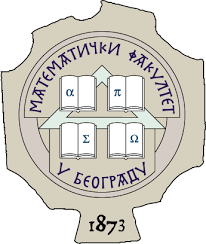
\includegraphics[width=0.3\textwidth]{matf_logo.png}
        
        \large{Београд, мај 2020}
        
    \end{center}
\end{titlepage}

\clearpage
{\mbox{}\vspace{15em}
\flushright                       
\Large \emph{Захваљујем се ментору проф. др Миодрагу Живковићу на инспирацији, помоћи и саветима при писању рада, као и члановима комисије доц. др Весни Маринковић и доц. др Ивану Чукићу на пажљивом читању и коментарима на тезу.} \par
\vfill
}

\clearpage
\textbf{Наслов мастер рада}: Игра ним\\

\textbf{Резиме}: Ним је игра за два играча са неколико гомила жетона. Број жетона и гомила је произвољан, тачније одређују их сами играчи. Постоје многе варијанте игре ним, које се од оригиналне верзије углавном разликују по томе што садрже бар једно додатно правило за игру. Мастер рад описује једну варијанту ове игре, под називом Витхофова игра. Приказана је подела позиција на добитне и изгубљене позиције, као и три начина да се одреди скуп изгубљених позиција, односно оптимални начин играња Витхофове игре. Програмски су реализовани описани алгоритми за одређивање изгубљених позиција и процењена њихова сложеност.\\

\textbf{Кључне речи}: ним, Витхофова игра, изгубљене позиције, добитне позиције, сто, жетони, стратегија

\clearpage

\tableofcontents

\newpage
\pagenumbering{arabic}

\section{Увод}
\label{sec:uvod}

Игра ним \cite{carls_buton} је игра са неколико гомила жетона за два играча. Број жетона и гомила је произвољан, тачније одређују их сами играчи. Играч који је на потезу може узети произвољан број жетона са једне гомиле, при чему мора узети бар један жетон и не сме узимати жетоне са више гомила. Играчи наизменично играју потезе. Постоје две варијанте игре: нормални и мизерни ним. У нормалном ниму побеђује играч који узме последњи жетон, док у мизерном губи играч који узме последњи жетон.

\begin{example}
На почетку партије на столу су три гомиле, са три, четири и пет жетона респективно. Партију играју два играча \textit{А} и \textit{Б}, \textit{А} игра први. 
\end{example}

Могући ток игре нормалног нима је приказан на слици \ref{fig:nimPrimer}.

\begin{figure}[H]
	\begin{center}
		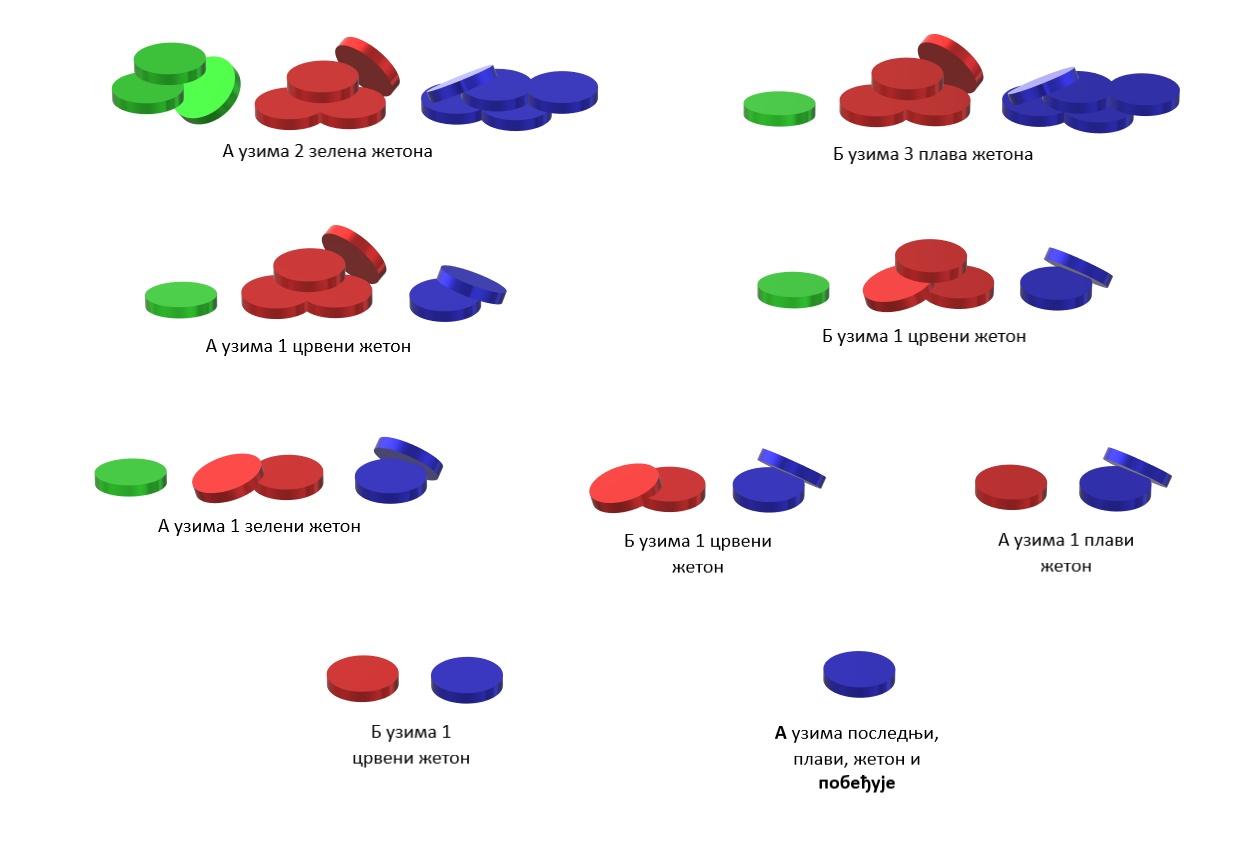
\includegraphics[width=\textwidth]{NimPrimer.png}
	\end{center}
	\caption{Ток игре ним}
	\label{fig:nimPrimer}
\end{figure}

Уколико се на столу налазе две гомиле, у зависности од броја жетона могући су следећи исходи нормалног нима:

\begin{itemize}
	\item На столу су две гомиле са по једним жетоном. Први играч мора да узме бар један жетон, чиме оставља другом играчу да узме последњи жетон и победи. У овој ситуацији очигледно је да \textbf{први играч гарантовано губи}.
	
	\item На столу су две гомиле, на првој један жетон, на другој два жетона. \textbf{Први играч има победничку стратегију}: уколико узме један жетон са гомиле где су два жетона (на слици \ref{fig:nimPrimer} узима 1 плави жетон), оставља следећем играчу две гомиле са по једним жетоном, што је за њега изгубљена позиција.
	
	\item На столу су две гомиле са по два жетона. Прва могућност јесте да први играч узме све са једне гомиле, чиме други играч истим тим потезом, узимајући све жетоне са друге гомиле побеђује. Друга могућност је да први играч узме један жетон, тако да је следеће стање игре заправо стање из претходног примера, у коме играч који је на потезу може да победи. У овој ситуацији \textbf{први играч губи} уколико други играч зна како да игра ним.
\end{itemize}

Сада би требало да је јасно да у овој игри нема неизвесности, односно да је свака позиција победничка или изгубљена за играча који је на потезу.

Постоје многе варијанте нима \cite{ho2011combinatorial, hitotsumatsu1968mathematics}, које се од оригиналне верзије углавном разликују по томе што садрже бар једно додатно правило за игру. Неке од варијанти су:
\begin{itemize}
	\item \textbf{Индекс k игра} (енг.{~\em Index-k nim}) у којој је дозвољено да играч у једном потезу узме жетоне са више гомила. 
	\item \textbf{Грандијева игра} (енг.{~\em Grundy's game}) се игра са једном гомилом жетона, где је једини дозвољен потез дељење текуће гомиле на две гомиле са различитим бројем жетона. Игра се завршава када остану гомиле са два или мање жетона.
	\item \textbf{Похлепни ним} (енг.{~\em Greedy nim}) у којој је дозвољено узимање жетона само са најбројније гомиле, а уколико је више таквих гомила онда је дозвољено узимање са произвољне најбројније гомиле.
	\item \textbf{Градитељски ним} (енг.{~\em Building nim}) се игра у две фазе. У првој фази играчи наизменично распоређују жетоне, на иницијално празне гомиле, све док се не распореде сви жетони. У другој фази се игра нормални ним. 
	\item \textbf{Витховофа игра} (енг.{~\em Wythoff's game}) се игра са две гомиле жетона; играчи наизменично узимају жетоне са једне или обе гомиле. Приликом узимања жетона са обе гомилe, рецимо $ k (> 0) $ са једне и $ l (> 0) $ са друге, мора да буде испуњен услов $ |k - l| < a $, где је $ a $ задати позитиван број који се одређује пре почетка партије и не мења се у току саме партије. Игра се завршава када број жетона на столу буде нула, а онај играч који је уклонио последњи жетон или жетоне је победник. Сваки играч када је на потезу мора да уклони бар један жетон. Забележено је да се ова игра играла у Кини  под именом "\begin{CJK}{UTF8}{gbsn}捡石子\end{CJK} jiǎn shízǐ", односно енг. {~\em picking stones} \cite{Yaglom}. Холандски математичар В. А. Витхоф (\textit{W. A. Wythoff}) је 1907. године објавио математичку анализу ове игре \cite{wythoff1907modification}. 
\end{itemize}

У наставку рада, у поглављу \ref{sec:optimalna_strategija} дат је приказ стратегије за нормални и мизерни ним у случају више гомила. У поглављу \ref{sec:optimalna_strategija_vithof} дата је основна класификација позиција на добитне и изгубљене, као и примери изгубљених позиција за Витхофову игру која је главна тема овог рада. Након чега је у поглављу \ref{sec:tri_Strategije} дат приказ три стратегије за победу у Витхофовој игри. На крају, у поглављу \ref{sec:implementacija_evaluacija} дат је приказ алгоритама написаниих у програмском језику C++, као и резултати њиховог извршавања.

\section{Варијанта нима са више гомила жетона}
\label{sec:optimalna_strategija}

Амерички математичар Чарлс Бутон (\textit{Charles Bouton}) је извршио комплетну математичку анализу ним игре 1902. године, односно одредио је све добитне и изгубљене позиције \cite{carls_buton}. Испоставља се да оцена позиције зависи од ексклузивне дисјункције (XOR) бинарно записаних бројева жетона на гомилама те да је потребно израчунати њихову ексклузивну дисјункцију (XOR) бит по бит, тј бинарну суму без преноса. 

\begin{example} 
	Нека су на столу дате две гомиле са пет и шест жетона, тада је њихова бинарна сума без преноса:	
	\begin{align*}
		5 = 1 0 1\\
		6 = 1 1 0\\
		----   \\
		3 = 0 1 1
	\end{align*}
\end{example}

\begin{theorem}
	\label{thm:pobeda}
	У нормалном ниму, позиција је изгубљена ако и само ако је бинарна сума без преноса бројева жетона једнака нули.
\end{theorem}

\begin{proof}
	Нека играч \textit{А} игра први, играч \textit{Б} други. На столу je $ n $ гомила са редом $ x_{1}, x_{2}, \ldots , x_{n} $ жетона, и нека је $ s $ ексклузивна дисјункција: 
	
	\begin{displaymath}
		s = x_{1} \oplus x_{2} \oplus x_{3} \ldots \oplus x_{n}.
	\end{displaymath}	
	Након што играч \textit{А} одигра свој потез, нека је $ t $ ексклузивна дисјункција жетона:
	\begin{displaymath}
		t = y_{1} \oplus y_{2} \oplus y_{3} \ldots \oplus y_{n}.
	\end{displaymath}
	 Уколико је $ s = 0 $, како се жетони могу узети само са једне гомиле, онда је за неко $ k $: $ x_{k} \neq y_{k} $ и за $ i \neq k $: $ x_{i} = y_{i} $, тако да је:	 
	 \begin{eqnarray*}
	 	t &=& 0 \oplus t \\
		  &=& s \oplus s \oplus t \\
		  &=& s \oplus (x_{1} \oplus x_{2} \oplus x_{3} \ldots \oplus x_{n}) \oplus (y_{1} \oplus y_{2} \oplus y_{3} \ldots \oplus y_{n}) \\
		  &=& s \oplus (x_{1} \oplus y_{1}) \oplus (x_{2} \oplus y_{2}) \oplus  \ldots \oplus (x_{n} + y_{n}) \\
		  &=& s \oplus (x_{k} \oplus y_{k}). 		 
	 \end{eqnarray*}
	 Дакле, уколико је $ s = 0 $, онда због $ x_{k} \neq y_{k} $ важи $ x_{k} \oplus y_{k} $ никад неће бити нула. Овим је доказано да уколико је тренутна бинарна сума без преноса нула, шта год противник одиграо сума постаје различита од $ 0 $.\\	 
	 Уколико je $ s \neq 0 $, нека је $ d $ позиција бита највеће тежине у $ s $ и нека је $ x_{k} $ гомила у којој је бит највеће тежине такође на позицији $ d $. Овакав бит увек постоји, јер бит највеће тежине из $ s $ долази од бита највеће тежине неких од бројева $ x_{1}, x_{2}, \ldots , x_{n} $ жетона. Ако се са гомиле $ x_{k} $ скине $ x_{k} - y_{k} $ жетона, где је $ y_{k} = s \oplus x_{k} $, бинарна сума без преноса постаје:
	 \begin{eqnarray*}
	 	t &=& s \oplus x_{k} \oplus y_{k} \\ 
	 	&=& s \oplus x_{k} \oplus s \oplus x_{k} \\
	 	&=& s \oplus s \oplus x_{k} \oplus x_{k} \\
	 	&=& 0.	 
	 \end{eqnarray*}	 
	 Овим је доказано да уколико тренутна бинарна сума без преноса није нула, увек је могуће направити потез тако да бинарна сума без преноса постане нула.
\end{proof}

\begin{example} 
	Нека су на столу дате три гомиле са седам, пет, дванаест жетона. Играч \textit{А} игра први, играч \textit{Б} игра други.	
		\begin{align*}
			7&		&   1 1 1&\\
			5&		&   1 0 1&\\
			+12&	& 1 1 0 0&\\
			---&	&--------&\\
			24&		& 1 1 1 0
		\end{align*}		
	У бинарном запису $ 1 1 1 0 $ бит највеће тежине је на позицији три, тако да играч \textit{А} узима са треће гомиле $ 1 1 0 0 - (1 1 0 0 \oplus  1 1 1 0) = 12 - 2 = 10 $  жетона.	
		\begin{align*}
			7&		&  	1 1 1&\\
			5&		&   1 0 1&\\
			+2&		&  	  1 0&\\
			---&	&--------&\\
			14&		&   0 0 0
		\end{align*}
	\textit{Б} може да узме на пример два жетона са друге гомиле.
		\begin{align*}
			7&		&   1 1 1&\\
			3&		&     1 1&\\
			+2&		&  	  1 0&\\
			---&	&--------&\\
			12&		&   1 1 0
		\end{align*}
	Тада \textit{А} треба да узме $ 1 1 1 - (1 1 0 \oplus 1 1 1) = 7 - 1 = 6 $  жетона са прве гомиле.
		\begin{align*}
			1&		&       1&\\
			3&		&     1 1&\\
			+2&		&  	  1 0&\\
			---&	&--------&\\
			6&		&     0 0
		\end{align*}
	\textit{Б} може да узме један жетон са треће гомиле.
		\begin{align*}
			1&		&       1&\\
			3&		&     1 1&\\
			+1&		&  	  	1&\\
			---&	&--------&\\
			5&		&     1 1
		\end{align*}
	\textit{А} треба да узме $ 1 1 - (1 1 \oplus 1 1) = 3 - 0 = 3 $ жетона са друге гомиле.
		\begin{align*}
			1&		&       1&\\
			+1&		&  	  	1&\\
			---&	&--------&\\
			2&		&       0
		\end{align*}
	На столу je паран број гомила са по једним жетоном, па \textit{Б} мора да узме један жетон са на пример прве гомиле.
		\begin{align*}
			1&		&  	  	1&\\
			---&	&--------&\\
			1&		&       1
		\end{align*}
	\textit{А} треба да узме последњи жетон и побеђује.\\
	Уколико је на столу паран број гомила са по једним жетоном, тада је бинарна сума без преноса нула. Играч који је на потезу може узети један жетон са било које гомиле, тако да на столу остаје непаран број гомила са по једним жетоном чиме бинарна сума без преноса постаје различита од нула, што на основу теореме \ref{thm:pobeda} противнику осигурава победу.
\end{example}

За мизерни ним се може пратити иста стратегија као у теореми \ref{thm:pobeda} све док не остану само гомиле са по једним жетоном. Тада је победа гарантована ако играч који је на потезу остави непаран број гомила са по једним жетоном.

\begin{example}
	Као и у претходном примеру, нека су на столу дате три гомиле са седам, пет, дванаест жетона. Играч \textit{А} игра први, играч \textit{Б} игра други.	
		\begin{align*}
			7&		&   1 1 1&\\
			5&		&   1 0 1&\\
			+12&	& 1 1 0 0&\\
			---&	&--------&\\
			24&		& 1 1 1 0
		\end{align*}		
	У бинарном запису $ 1 1 1 0 $ бит највеће тежине је на позицији три, тако да играч \textit{А} узима са треће гомиле $ 1 1 0 0 - (1 1 0 0 \oplus  1 1 1 0) = 12 - 2 = 10 $  жетона.	
		\begin{align*}
			7&		&  	1 1 1&\\
			5&		&   1 0 1&\\
			+2&		&  	  1 0&\\
			---&	&--------&\\
			14&		&   0 0 0
		\end{align*}
	\textit{Б} може да узме на пример два жетона са друге гомиле.
		\begin{align*}
			7&		&   1 1 1&\\
			3&		&     1 1&\\
			+2&		&  	  1 0&\\
			---&	&--------&\\
			12&		&   1 1 0
		\end{align*}
	Тада \textit{А} треба да узме шест жетона са прве гомиле.
		\begin{align*}
			1&		&       1&\\
			3&		&     1 1&\\
			+2&		&  	  1 0&\\
			---&	&--------&\\
			6&		&     0 0
		\end{align*}
	\textit{Б} може да узме један жетон са треће гомиле.
		\begin{align*}
			1&		&       1&\\
			3&		&     1 1&\\
			+1&		&  	  	1&\\
			---&	&--------&\\
			5&		&     1 1
		\end{align*}	
	У позицији у којој само на једној гомили има више од једног жетона је преокрет стратегије за мизерни ним. Тако да \textit{А} треба да узме два жетона са друге гомиле, како би оставио непаран број гомила са по једним жетоном и победио.
		\begin{align*}
			1&		&		1&\\
			1&		&       1&\\
			+1&		&  	  	1&\\
			---&	&--------&\\
			3&		&       1
		\end{align*}
	\textit{Б} може да узме један жетон са на пример прве гомиле.
		\begin{align*}
			1&		&		1&\\
			1&		&  	  	1&\\
			---&	&--------&\\
			2&		&       0
		\end{align*}
	\textit{А} може да узме један жетон са друге гомиле.
		\begin{align*}
			1&		&  	  	1&\\
			---&	&--------&\\
			1&		&       1
		\end{align*}
	\textit{Б} треба да узме последњи жетон и губи.
\end{example}

\section{Оптимална стратегија за Витхофову игру}
\label{sec:optimalna_strategija_vithof}

Било која позиција се може представити паром бројева $ (x, y) $, где је $ x \le  y $. Овде $ x $ и $ y $ представљају бројеве жетона на две гомиле. У случају класичне Витхофове игре ( $ a = 1 $ што значи да ако играч узима жетоне са обе гомиле, број узетих жетона мора бити једнак) игра се еквивалентно може описати и као игра са краљицом на шаховској табли \cite{larsson2010restrictions}: негде на шаховској табли је краљица, играч који је на потезу може да помери краљицу произвољан број корака у правцу југа, запада, или југозапада. Победник је играч који први помери краљицу у доњи леви угао табле (при чему су координате доњег левог угла (0, 0)). Све могуће позиције могу се разврстати у две категорије, добитне и изгубљене.

\begin{definition}
	У изгубљеној позицији, играч који је на потезу губи, док наредни играч може да победи шта год одиграо противник. У добитној позицији, играч који је на потезу може да победи без обзира како игра противник.
\end{definition}

\begin{lemma}
	Класификација позиција на добитне и изгубљене се дефинише рекурзивно на следећи начин:
		\begin{enumerate}
			\item $ (0, 0) $ је по дефиницији изгубљена позиција, јер играч који је на потезу не може да одигра ниједан валидан потез, па је његов противник победник.
			\item Било која позиција из које је у једном потезу достижна изгубљена позиција је добитна позиција.
			\item Ако сваки потез води ка некој добитној позицији, онда је то изгубљена позиција.
		\end{enumerate}	
\end{lemma}

\begin{proof}
	Позиција $ (0, 0) $ је изгубљена позиција за играча који је на потезу, јер нема више жетона на столу и не постоји ниједан валидан потез који противник може направити. Jасно је да су позиције $ (x, x) $ и $ (0, x) $ добитне за свако $ x > 0 $,  јер се из њих једним потезом може прећи у позицију $ (0, 0) $, која је изгљубљена позиција за противника.\\
	%Нека су $ (x_{n}, y_{n}) $, $ x_{n} \le y_{n} $ и $ (x_{m}, y_{m}) $, $ x_{m} \le y_{m} $ изгубљене позиције и $ n > m $. Како је $ y_{n} = x_{n} + an $ и $ y_{m} = x_{m} + am $. Одузимањем $ y' = y_{n} - y_{m} = x_{n} + an - x_{m} - am = x_{n} - x_{m} + a(n - m) = x' + a(n - m) $, добија се $ y' - x' = a(n - m) \ge a $, тако да не постоји валидан потез из $ (x_{n}, y_{n}) $ у $ (x_{m}, y_{m}) $, уколико је $ (x_{m}, y_{m}) $ изгубљена позиција.
	Дакле, из изгубљене позиције достижна је у једном потезу добитна позиција.
\end{proof}

Да би се Витхофова игра играла на најбољи могући начин, потребно је знати две ствари:
\begin{itemize}
	\item Препознати природу тренутне позиције, да ли је добитна или изгубљена.
	\item Уколико је тренутна позиција добитна, треба одредити следећи потез тако да се противник нађе у изгубљеној позицији.
\end{itemize}

Класификација позиција на добитне и изгубљене је важна, јер ако је тренутна позиција добитна, постоји потез који води ка изгубљеној позицији, а тај потез се може одредити. Са друге стране, ако је тренутна позиција изгубљена, не може се урадити ништа, само одиграти произвољан валидан потез и надати се да ће противник одиграти погрешан потез, с обзиром на то да се у једном потезу из изгубљене позиције стиже у добитну позицију, из које противник може да победи ако зна да одреди изгубљену позицију. 

\begin{example}
	За $ a = 1 $:
		\begin{itemize}
			\item прва изгубљена позиција је $ (1, 2) $, јер ако играч узима жетоне само са једне гомиле у једном потезу достижне су само позиције:
				\begin{displaymath}
					(1, 1), \text{и}\ (0, 2),
				\end{displaymath}
			док ако играч узима жетоне са обе гомиле, рецимо $ k (> 0) $ са једне и $ l (> 0) $ са друге, мора да буде испуњен услов $ |k - l| < 1 $, тако да играч може узети $ k = 1 $ и $ l = 1 $ жетона, па се у једном потезу може доћи у позицију:
				\begin{displaymath}
					(0, 1)
				\end{displaymath}
			Следећи играч, из позиција $ (0, 1) $ и $ (0, 2) $, узимањем свих жетона са гомиле где је број жетона већи од $ 0 $ може доћи само у позицију $ (0, 0) $, а из позиције $ (1, 1) $ узимањем по једног жетона са обе гомиле достижна је само позиција $ (0, 0) $.\\
			Дакле, пошто је из позиција $ (0, 1),\ (0, 2) $ и $ (1, 1) $ у једном потезу достижна изгубљена позиција $ (0,0) $ оне су добитне позиције.
			\item следећа изгубљена позиција је $ (3, 5) $, јер ако играч узима жетоне само са једне гомиле достижне су позиције:
				\begin{displaymath}
					(3, 4),\ (3, 3),\ (2, 5),\ (1, 5)\  \text{и}\ (0, 5),
				\end{displaymath}
			док ако узима жетоне са обе гомиле, у једном потезу достижне су позиције:
				\begin{displaymath}
					(2, 4),\ (1, 3)\ \text{и}\ (0, 2)
				\end{displaymath}
			Из позиција $ (3, 4),\ (3, 3),\ (2, 5),\ (1, 5),\ (0, 5),\ (2, 4)\ (1, 3) $ и $ (0, 2) $ у једном потезу достижне су позиције $ (0, 0) $ или $ (1, 2) $ па су оне добитне.
		\end{itemize}
		Може се приметити, да је за $ i $-ту изгубљену позицију, уколико је $ i = 1...n $, разлика бројева у пару једнака $ i $, и да је унија низа првих и низа других компоненти парова једнака скупу првих $ n $ природних бројева. Такође се може приметити да су компоненте пара бројева изгубљених позиција (сем $ (0, 0) $) дисјунктне, ово тврђење је показано касније у секцији \ref{sec:tri_Strategije}, теорема \ref{thm:reukrzivna_strategija}.\\
		Изгубљене позиције приказане су у табели \ref{tab:a_1_Ppozicije} и на слици \ref{fig:p_positions_a=1} (црвена поља).
\end{example}
	
\begin{table}[h!]
	\caption{Приказ првих $ 11 $ изгубљених $ (A, B) $ позиција за $ a = 1 $}
	\label{tab:a_1_Ppozicije}
	\begin{center}
		\begin{tabular}{  c | c | c }
			{\textbf{n}} &  {\textbf{A}} &  {\textbf{B}} \\
			\hline
			0 & 0 & 0 \\
			1 & 1 & 2 \\
			2 & 3 & 5 \\
			3 & 4 & 7 \\
			4 & 6 & 10 \\
			5 & 8 & 13 \\
			6 & 9 & 15 \\
			7 & 11 & 18 \\
			8 & 12 & 20 \\
			9 & 14 & 23 \\
			10 & 16 & 26\\
			11 & 17 & 28\\ 
		\end{tabular}
	\end{center}
\end{table}

\begin{figure}[H]
	\begin{center}
		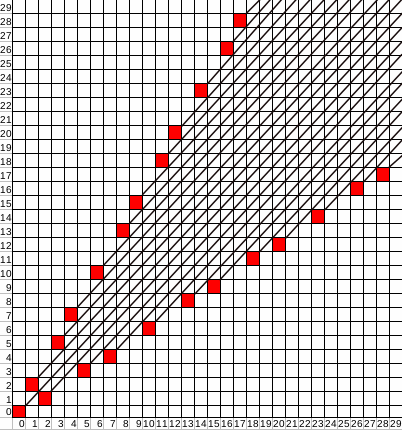
\includegraphics[width=350px, height=350px]{p_positions_a=1.png}
	\end{center}
	\caption{Визуелни приказ изгубљених позиција за $ a = 1 $}
	\label{fig:p_positions_a=1}
\end{figure}

\begin{example}
	За $ a = 2 $, изгубљене позиције приказане су у табели \ref{tab:a_2_Ppozicije} и на слици \ref{fig:p_positions_a=2} (црвена поља).
\end{example}

\begin{table}[h!]
	\caption{Приказ првих $ 9 $ изгубљених $ (A, B) $ позиција за $ a = 2 $}
	\label{tab:a_2_Ppozicije}
	\begin{center}
		\begin{tabular}{  c | c | c }
			{\textbf{n}} &  {\textbf{A}} &  {\textbf{B}} \\
			\hline
			0 & 0 & 0 \\
			1 & 1 & 3 \\
			2 & 2 & 6 \\
			3 & 4 & 10 \\
			4 & 5 & 13 \\
			5 & 7 & 17 \\
			6 & 8 & 20 \\
			7 & 9 & 23 \\
			8 & 11 & 27 \\
			9 & 12 & 30 \\
			10 & 14 & 34\\ 
		\end{tabular}
	\end{center}
\end{table}

\begin{figure}[H]
	\begin{center}
		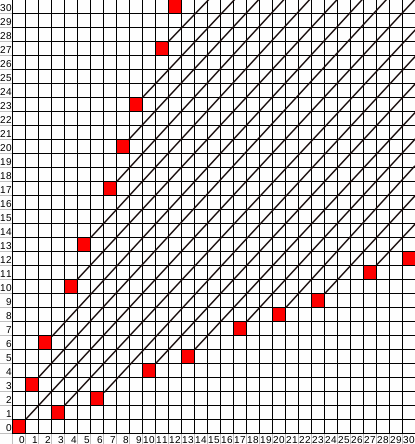
\includegraphics[width=350px, height=350px]{p_positions_a=2.png}
	\end{center}
	\caption{Визуелни приказ изгубљених позиција за $ a = 2 $}
	\label{fig:p_positions_a=2}
\end{figure}

\begin{example}
	У варијанти $ a = 1 $ игра се може еквивалентно описати као игра са краљицом на шаховској табли. Дозвољено је краљицу померати за произвољан број поља ка југу, југозападу и западу у односу на текућу позицију. На столу је табела $ 10\times10 $, на позицији $ (0, 0) $ је циљ. Игру играју два играча \textit{А} и \textit{Б}, померајући наизменично краљицу од почетне позиције $ (x,y) $. Победник је играч који први доведе краљицу до циља. На табли су све позиције $ (x, y) $, а не само $ x \leq y $.
	
	Играч \textit{А} игра први, \textit{Б} други. На слици \ref{fig:sahovska_tabla_pozicije_a_1} је дат приказ изгубљених позиција(зелена поља) и како се до њих може доћи (плаве и црвене стрелице). Слика \ref{fig:sahovska_tabla_pozicije_a_1} је аналогна претходним дијаграмима (табела \ref{tab:a_1_Ppozicije} и \ref{fig:p_positions_a=1}). Уколико је краљица на позицији $ (0, y), (x,0) $ или $ (x,x) $, при чему је $ x > 0, y > 0 $, играч \textit{А}, уколико игра како треба, у једном потезу може довести краљицу до циља и победити. Позиција $ (1, 2) $ је изгубљена позиција, јер ако играч \textit{А} краљицу доведе у ову позицију, играч \textit{Б} из позиције $ (1, 2) $ краљицу може да помери само у једну од позиција: $ (1, 1) $, $ (1, 0) $, $ (0, 2) $ или $ (0, 1) $. Следећа оваква позиција је $ (3, 5) $. Уопште, уколико је краљица на позицији, из које се плавом или црвеном стрелицом може прећи у зелено поље, играч \textit{А} може краљицу једним потезом довести до изгубљене позиције, са које су достижне само добитне позиције и са којих играч \textit{А} може директно довести краљицу до циља или је померити на неку од преосталих изгубљених позиција ближих циљу. Уколико из тренутне позиције ниједан валидан потез не води до зеленог поља, онда је та позиција изгубљена. На слици \ref{fig:sahovska_tabla_pozicije_a_1} то су управо зелена поља и поље $ (0, 0) $, ово важи јер из, на пример, позиције $ (3, 5) $ у једном потезу није достижно ниједно друго зелено поље.
\end{example}
 
\begin{figure}[H]
	\begin{center}
		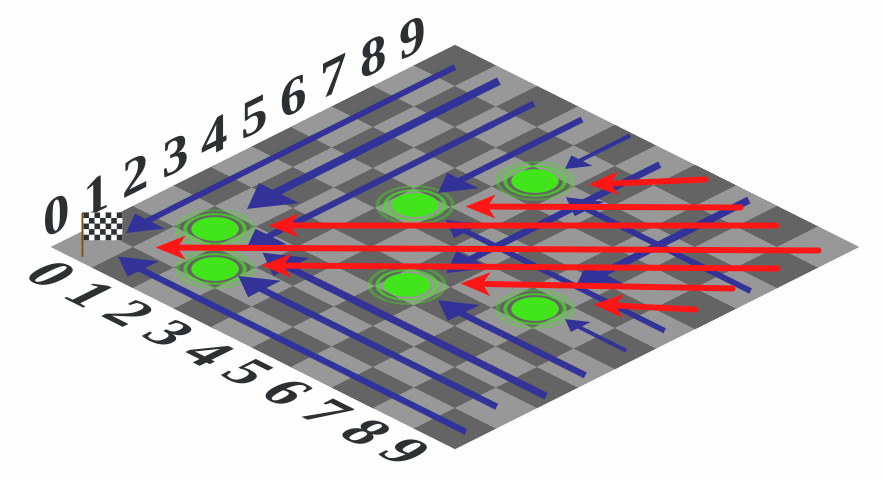
\includegraphics[width=\textwidth]{10x10_a1.png}
	\end{center}
	\caption{Приказ изгубљених позиција на табли $ 10 \times 10 $ за $ a = 1 $}
	\label{fig:sahovska_tabla_pozicije_a_1}
\end{figure}

Свака позиција је добитна или изгубљена; лако се види како се, корак по корак, за сваку позицију може установити тип. У наставку следи приказ три стратегије за одређивање типова свих позиција: рекурзивна, алгебарска и аритметичка стратегија.

\section{Три еквивалентне формулације стратегије за Витхофову игру}
\label{sec:tri_Strategije}

Израелски математичар Авзри Сигмуд Френкел (Aviezri Siegmund Fraenkel) je 1982. године у свом раду \cite{10.2307/2321643} дао приказ три математичке стратегије за победу у Витхофовој игри. У овом поглављу следи опис прво рекурзивне, потом алгебарске и на крају аритметичке стратегије.

\subsection{Рекурзивна стратегија}

Рекурзивни поступак за одређивање изгубљених позиција заснива се на оператору $ \mex $.

\begin{definition}
	\label{def:mex}
	$\mex(A)$ означава најмањи природни број који није у скупу $ A $, тј. $ \mex(\emptyset)=0 $ и
$ \mex(A)=\min\{i | i\notin A\} $.
\end{definition}

Описани начин добијања изгубљених позиција $ (A_{n}, B_{n}) $, може се поједноставити, што показује следећа теорема. 

\begin{theorem} [Рекурзивна карактеризација изгубљених позиција]
	\label{thm:reukrzivna_strategija}
	Нека је 
	\begin{eqnarray}
		&A_{n} = &\mex \{ A_{i}, B_{i} : i < n \}\\
		&B_{n} = &A_{n} + an
	\end{eqnarray}
	Тада је скуп свих изгубљених позиција
	$ P = \cup_{i=0}^{\infty} \{(A_{i},B_{i})\} $.
\end{theorem}

\begin{proof}
	
	Из израза за $ A_{n} $ и $ B_{n} $ у формулацији теореми следи да ако је $ A = \cup_{n=1}^{\infty}\{A_{n}\} $ и  $ B = \cup_{n=1}^{\infty}\{B_{n}\} $ онда су $ A_{n} $ и $ B_{n} $ \textbf{комплементарни} скупови, тј. $ A \cup B = Z^{+} $ скуп целих позитивних бројева  и $ A \cap B = \emptyset $. Тврђење $ A \cup B = Z^{+} $ важи јер из израза за $ A_{n} $ следи да ниједан број не може бити испуштен, а $ A \cap B = \emptyset $ јер у случају да је $ A_{n} = B_{m} $, и $ n > m $, следи да је $ A_{n} $ $ \mex $ скупа који садржи $ B_{m} = A_{n} $ што је у супротности са изразом за $ A_{n} $ из формулације теореме. Случај када је $ n \leq m $ је немогућ јер је тада $ B_{m} = A_{m} + am \geq  A_{n} + an > A_{n} $. 
	
	Да би се доказала теорема остаје да се докаже:
	\begin{itemize}
		\item да се из произвољне позиције $ (A_{n}, B_{n}) $ не може доћи у неку претходну позицију $ (A_{i}, B_{i}), i < n $
		\item да се из позиције $ (x, y) \notin P, x < y $, може прећи само у неку изгубљену позицију $ (A_{n}, B_{n}) $.
	\end{itemize}
	
	Из изгубљене позиције, једним потезом може се прећи само у добитну позицију. Из позиције $ (A_{n}, B_{n}) $ узимањем жетона само са једне гомиле прелази се у другу позицију, при чему нова позиција не може бити облика $ (A_{i}, B_{i}) $. Ово следи из чињенице да су  $ A_{n} $ и $ B_{n} $ комплементарни скупови. Уколико се жетони узимају са обе гомиле, такође се прелази у позицију која није облика $ (A_{i}, B_{i}) $. У противном би за нову позицију $ (A_{i}, B_{i}) $ морало да важи $ |(B_{n} - B_{i}) - (A_{n}-A_{i})| < a $. Међутим из једнакости $ B_{n} - A_{n} = an $ следи $ |(n-i)a| < a $, тј. $ i = n $, што је контрадикција. 
	
	Из добитне позиције једним потезом може се прећи само у изгубљену позицију. За позицију $ (x, y), x \le y $, која није изгубљена позиција облика $ (A_{i}, B_{i}), i \ge 0 $ и где су $ A_{n} $ и $ B_{n} $ комплементарни скупови, може се сматрати да је $ x = B_{n} $, или је $ x = A_{n} $, за неко $ n \ge 0 $. Тако су позиције у које се може прећи из $ (x, y) $:
	
	\begin{itemize}
		\item \label{case:slucaj1} Случај 1: Ако је $ x = B_{n} $ онда се из позиције $ (x = B_{n}, y) $ може једним потезом (скидањем жетона са гомиле на којој је $ y $ жетона) прећи у изгубљену позицију $ (A_{n}, B_{n}) $ 
		\item \label{case:slucaj2} Случај 2: Ако је $ x = A_{n} $ и $ y > B_{n} $, онда се смањивањем $ y $ може доћи у позицију $ (A_{n}, B_{n}) $. У противном, ако је $ A_{n} \le y < B_{n} $ онда се смањивањем $ x $ и $ y $ може прећи у позицију $ (A_{m}, B_{m}) $, где је $ m = \lfloor \frac{d}{a} \rfloor $ и $ d = y - x $. Заиста, из $ d = y - A_{n} < B_{n} - A_{n} = an $, следи да је  $ m = \lfloor \frac{d}{a} \rfloor \le \frac{d}{a} < n $. Поред тога важи неједнакост $ y = A_{n} + d \ge A_{m} + am = B_m $. Из позиције $ (x, y) $ смањивањем обе компоненте прелази се у позицију $ (A_{m}, B_{m}) $, при чему за смањење компоненти важи неједнакост $ |(y - B_{m}) - (x - A_{m})| = d - am < a $.
	\end{itemize}
	
\end{proof}

\begin{example}
	Уколико је $ a = 2 $ и тренутна позиција $ (x, y) $ није изгубљена позиција, следе примери одређивања наредног потеза коришћењем списка изгубљених позиција $ (A_{n}, B_{n}) $ из табеле \ref{tab:a_2_Ppozicije}:
	\begin{itemize}
		\item Нека је тренутна позиција $ (x, y) = (17, 29) $. Како је $ B_{5} = 17 $, то се из позиције $ (17, 29) $ једним потезом уклањајући $ 22 $ жетона са друге гомиле прелази у позицију $ (A_{5}, B_{5}) = (7, 17) $. 
		\item Нека је тренутна позиција $ (x, y) = (11, 29) $. Како је $ A_{8} = 11 $ и $ 29 > B_{8} = 27 $, то се из позиције $ (11, 29) $ једним потезом уклањајући $ 2 $ жетона са друге гомиле прелази у позицију $ (A_{8}, B_{8}) = (11, 27) $.
		\item Нека је тренутна позиција $ (x, y) = (11, 25) $. Како је $ A_{8} = 11 $ и $ 25 < B_{8} = 27 $, то се из позиције $ (11, 25) $ једним потезом уклањајући $ 2 $ жетона са прве гомиле и $ 2 $ са друге гомиле прелази у позицију $ (A_{7}, B_{7}) = (9, 23) $.
	\end{itemize}
\end{example}

Уколико је тренутна позиција $ (x, y) $, $ 0 \leq x \leq y $, прво је потребно формирати табелу са најмање $ n $ изгубљених позиција, тако да је $ A_{n} = x $ или $ B_{n} = x $. Пошто зa елементе из скупа $ A $ важи $ A_{n} \leq 2n $, то је за ово рачунање потребно највише $ O(x) $ поређења, и $ O(x) $ меморијског простора. Бинарном претрагом се у табели проналазе $ A_{n} $ или $ B_{n} $ тако да је $ A_{n} = x $ или $ B_{n} = x $. Према томе, укупно време потребно за формирање табеле изгубљених позиција је $ O(x) $.

\subsection{Алгебарска стратегија}

Испоставља се да се све изгубљене позиције $ (A_{n}, B_{n}) $ могу експлицитно изразити на следећи начин $ A_{n} = \lfloor \alpha \cdot n \rfloor, B_{n} = \lfloor \beta \cdot n \rfloor $, где је:

\begin{eqnarray}
	&\alpha = &\frac{2 - a + \sqrt{a^2 + 4}}{2} \label{def:alpha}\\  
	&\beta = &\alpha + a \label{def:beta}.
\end{eqnarray}
Овде су $ \alpha $ и $ \beta $ ирационални за свако $ a > 0 $, и $ \alpha $ је позитиван корен једначине $ \alpha^{-1} + \beta^{-1} = 1 $. Из ове једнакости следи неједнакост
$ 1<\alpha<2 $, јер због $ \beta^{-1} = (\alpha+a)^{-1} < \frac{1}{2 }$ мора да буде $ \alpha^{-1} > \frac{1}{2} $.

Ако је $ \alpha $ произвољан ирационални број, онда се целобројни растући низ $ \lfloor \alpha \cdot 0 \rfloor, \lfloor \alpha \cdot 1 \rfloor, \ldots \lfloor \alpha \cdot n \rfloor $ зове Бетијев низ (\textit{{Beatty}}), за $ 0 \ldots n $, општи члан низа је $ \lfloor \frac{2-a+\sqrt{a^{2}+4}}{2} \cdot i \rfloor $.

Најпре следи доказ општег тврђења о Бетијевим низовима.

\begin{lemma}
	\label{lemma:alg_komplementarnost}
	Нека су $ \alpha $ и $ \beta $ позитивни ирационални бројеви који задовољавају услов $ \alpha^{-1} + \beta^{-1} = 1 $ и нека је 
	\begin{eqnarray*} 
		&A^{'}_{n}= &\lfloor \alpha \cdot n \rfloor\\
		&B^{'}_{n} = &\lfloor \beta \cdot n \rfloor\\
		&A^{'} = &\cup_{n=1}^{\infty}\{A^{'}_{n}\}\\
		&B^{'} = &\cup_{n=1}^{\infty}\{B^{'}_{n}\}
	\end{eqnarray*}
	Тада су $ A^{'} $ и $ B^{'} $ комплементарни скупови.
\end{lemma}

\begin{proof}
	Довољно је показати да се тачно један елемент уније $ A^{'} \cup B^{'} $ налази у интервалу $ [N,N+1) $, за сваки позитиван број $ N $, тј. довољно је да одредимо колико има бројева из скупа $ A^{'} \cup B^{'} $ који су мањи од $ N $, ако је $ N > 1 $. Бројева из $ A^{'} $ мањих од $ N $ има $ \left\lfloor \frac{N}{\alpha} \right\rfloor $. Бројева из $ B^{'} $ мањих од $ N $ има $ \left\lfloor \frac{N}{\beta} \right\rfloor $. Сабирањем двоструких неједнакости:
		\begin{eqnarray*}
			&\frac{N}{\alpha} - 1 < \left\lfloor \frac{N}{\alpha} \right\rfloor < \frac{N}{\alpha}\\
			&\frac{N}{\beta} - 1 < \left\lfloor \frac{N}{\beta} \right\rfloor < \frac{N}{\beta}
		\end{eqnarray*}	
	добија се:
		\begin{displaymath}
		N - 2 < \left\lfloor \frac{N}{\alpha} \right\rfloor + \left\lfloor \frac{N}{\beta} \right\rfloor < N
		\end{displaymath} 	
	Oдавде следи да је $ \left\lfloor \frac{N}{\alpha} \right\rfloor + \left\lfloor \frac{N}{\beta} \right\rfloor = N - 1 $, тј. $ N - 1 $ бројева из уније $ A^{'} \cup B^{'} $ је мање од $ N $. Слично важи и да је $ N $ бројева из $ A^{'} \cup B^{'} $ мање од $ N + 1 $. Према томе, тачно $ N - (N - 1) = 1 $ елемент те уније припада интервалу $ [N,N+1) $.
\end{proof}

\begin{lemma}
	\label{lemma:n}
	Ако је $ \lfloor \alpha \cdot n \rfloor = x $, онда је:
		\begin{eqnarray*}
			n = \left\lfloor \frac{x+1}{\alpha} \right\rfloor
		\end{eqnarray*}
\end{lemma}

\begin{proof}
	Ово следи из двоструке неједнакости $ \frac{x}{\alpha}<n<\frac{x+1}{\alpha} $ јер је неједнакост $ \frac{x+1}{\alpha} - \frac{x}{\alpha} < 1 $, а интервал дужине мање од 1 може да садржи највише један цели број.
\end{proof}

\begin{lemma}[Алгебарска карактеризација изгубљених позиција] Нека су $ \alpha $ и $ \beta $ дефинисани једнакостима \eqref{def:alpha}, \eqref{def:beta}. Тада је скуп свих изгубљених позиција $ P = \cup_{n=0}^{\infty} \{(\lfloor \alpha \cdot n \rfloor, \lfloor \beta \cdot n \rfloor)\} $.
\end{lemma}

\begin{proof}
	Уочимо да је $ A^{'}_{0} = 0, B^{'}_{0} = 0 $ и $ B^{'}_{n} - A^{'}_{n} = an $. Такође како су $ A^{'}_{n} $ и $ B^{'}_{n} $ растући и комплементарни скупови, важи још и да је $ A^{'}_{n} = \mex \{ A^{'}_{i}, B^{'}_{i} : i < n \} $. Из ове чињенице индукцијом следи да је $ A^{'}_{n} = A_{n} $ и $ B^{'}_{n} = B_{n}  $ за $ n \ge 0 $.
\end{proof}

Нека је $ (x, y), x \leq y $ тренутна позиција. Тада је $ x = \lfloor n \alpha \rfloor = A_{n} $, где је $ n = \lfloor \frac{(x+1)}{\alpha} \rfloor $ или је $ x = \lfloor n \beta \rfloor = B_{n} $, где је $ n = \lfloor \frac{(x+1)}{\beta} \rfloor $, видети доказ теореме \ref{thm:reukrzivna_strategija} и леме \ref{lemma:n}. На пример, ако је $ x = \lfloor n \alpha \rfloor = A_{n} $, и $ \lfloor n \alpha \rfloor < y < \lfloor n \beta \rfloor $ онда се смањивањем $ x $ и $ y $ може прећи у позицију $ (\lfloor m \alpha \rfloor, \lfloor m \beta \rfloor) $, где је $ m = \lfloor \frac{d}{a} \rfloor $ и $ d = y - x $, при чему за смањење компоненти важи неједнакост $ |(y - \lfloor m \beta \rfloor) - (x - \lfloor m \alpha \rfloor)| = d - am < a $.

\begin{example}
	У специјалном случају за $ a = 1 $ важи $ \alpha = \frac{1 + \sqrt{5}}{2} $, што је вредност позната као златни пресек.\\	
	Низ $ \lfloor \alpha \cdot n \rfloor $ се назива доњи Витхофов низ ($ A_{n} $):
	$ 1, 3, 4, 6, 8, 9, 11, 12, 14, 16 \ldots $. Низ $ \lfloor (\alpha + 1) n \rfloor $ се назива горњи Витхофов низ ($ B_{n} $):
	$ 2, 5, 7, 10, 13, 15, 18, 20, 23, 26 \ldots $
\end{example}

\subsection{Аритметичка стратегија}

Нека је $ \alpha $ ирационалан број, који задовољава услов $ 1 < \alpha < 2 $. Број $ \alpha $ се може једнозначно представити бесконачним верижним разломком облика \cite{hardy2008introduction, olds1963continued}:
\begin{displaymath}
	\alpha = a_{0} + \frac{1}{a_{1} + \frac{1}{a_{2} + \frac{1}{a_{3} + \ldots}}}.
\end{displaymath}
Чланови низа $ a_{n} $ добијају се поступком сличним Еуклидовом алгоритму, тј. број $ \alpha $ одређује низ $ a_{n} $. Обрнуто сваки бесконачни верижни развoј једнозначно одређује ирационални број. При томе, ако је $ n > 1 $, онда је $ a_{n} > 1 $.
Рационални бројеви $ C_{0} = [a_{0}] = a_{0},\ C_{1} = [a_{0}, a_{1}] = a_{0} + \frac{1}{a_{1}},\ C_{2} = [a_{0}, a_{1}, a_{2}] = a_{0} + \frac{1}{a_{1} + \frac{1}{a_{2}}},\ C_{3} = [a_{0}, a_{1}, a_{2}, a_{3}] = a_{0} + \frac{1}{a{1} + \frac{1}{a_{2} + \frac{1}{a_{3}}}}, \ldots $ где је $ a_{i} > 0 $ и $ i > 0 $ су конвергенти броја $ \alpha $.
Испоставља се да конвергенти броја $ \alpha $ конвергирају броју $ \alpha $:
\begin{displaymath}
	\alpha = \lim\limits_{n \rightarrow \infty} C_{n} = \lim\limits_{n \rightarrow \infty} [a_{0}, a_{1}, a_{2}, a_{3}, \ldots, a_{n}].
\end{displaymath}
Другим речима, бесконачни верижни разломак $ [a_{0}, a_{1}, a_{2}, a_{3}, \ldots] $ једнак је броју $ \alpha $. Доказ ове чињенице следи у наставку.

\begin{definition}
	\label{def:p_q_nizovi}
	Нека су $ p_{n} $ и $ q_{n} $ узајамно прости бројеви такви да је:
	\begin{displaymath}
		\frac{p_{n}}{q_{n}} = [a_{0}, a_{1}, a_{2}, a_{3}, \ldots, a_{n}].
	\end{displaymath}	
\end{definition}

\begin{lemma}
	\label{lemmma:p_q_nizovi}
	Нека је $ [a_{0}, a_{1}, a_{2}, \ldots] $ верижни развој броја $ \alpha $ и за низове $ p $ и $ q $ важи следећа рекурентна релација:
	\begin{eqnarray}
		p_{-1} = 1,\ p_{0} = a_{0},\ p_{n} = a_{n}p_{n-1} + p_{n-2},\ (n \geq 1 )\\
		q_{-1} = 0,\ q_{0} = 1,\ q_{n} = a_{n}q_{n-1} + q_{n-2},\ (n \geq 1 ).
	\end{eqnarray}
	Тада су конвергенти броја $ \alpha $ дати изразом:	
	\begin{eqnarray}
		C_{n} = \frac{p_{n}}{q_{n}} = \frac{a_{n}p_{n-1} + p_{n-2}}{a_{n}q_{n-1} + q_{n-2}}.
	\end{eqnarray}
\end{lemma}

\begin{proof}	
	Индукцијом се показује да се бројиоци и имениоци конвергената могу одредити полазећи од $ p_{0} = a_{0},\  q_{0} = 1 $ и $ p_{1} = a_{1}a_{0} + 1,\ q_{1} = a_{1} $ на основу рекурентних релација $ p_{i} = a_{i}p_{i-1} + p_{i-2},\ q_{i} = a_{i}q_{i-1} + q_{i-2},\ i = 1, 2, \ldots $.\\
	Прелаз у доказу индукцијом заснива се на замени $ a_{i} $ у верижном разломку $ \frac{p_{i}}{q_{i}} $, са $ a_{i} + \frac{1}{a_{i} + 1} $
	у $ \frac{p_{i+1}}{q_{i+1}} $.\\
	По индуктивној хипотези је $ p_{i} = a_{i}p_{i-1} + p_{i-2}, q_{i} = a_{i}q_{i-1} + q_{i-2} $ и $ \frac{p_{i}}{q_{i}} = [a_{0}, a_{1}, , a_{2}, , a_{3}, \ldots, a_{i}] $. Због тога је:	
	\begin{eqnarray*}
		\frac{p_{i+1}}{q_{i+1}} &=& [a_{0}, a_{1}, , a_{2}, , a_{3}, \ldots, a_{i}, a_{i+1}]\\
		&=& [a_{0}, a_{1}, , a_{2}, , a_{3}, \ldots, a_{i}, a_{i} + \frac{1}{a_{i+1}}] \\
		&=& \frac{(a_{i} + \frac{1}{a_{i+1}})p_{i-1} + p_{i-2}}{(a_{i} + \frac{1}{a_{i+1}})q_{i-1} + q_{i-2}} \\
		&=& \frac{a_{i+1}a_{i}p_{i-1} + p_{i-1} + a_{i+1}p_{i-2}}{a_{i+1}a_{i}q_{i-1} + q_{i-1} + a_{i+1}q_{i-1}}\\
		&=& \frac{a_{i+1}(a_{i}p_{i-1} + p_{i-2}) + p_{i-1}}{a_{i+1}(a_{i}q_{i-1} + q_{i-2}) + q_{i-1}}\\
		&=& \frac{a_{i+1}p_{i} + p_{i-1}}{a_{i+1}q_{i} + q_{i-1}}. 
	\end{eqnarray*}
\end{proof}

\begin{lemma}
	\label{lemma:svojstva_p_q_1}
	Бројеви $ p_{n} $ и $ q_{n} $ задовољавају услов:	
	\begin{eqnarray}
		\label{c.f_svojstvo_1} p_{n}q_{n-1} - p_{n-1}q_{n} = (-1)^{n}.
	\end{eqnarray}	
\end{lemma}

\begin{proof}
	\begin{eqnarray*}
		p_{n}q_{n-1} - p_{n-1}q_{n} &=& (a_{n}p_{n-1} + p_{n-2})q_{n-1} - p_{n-1}(a_{n}q_{n-1} + q_{n-2})\\
									&=& a_{n}p_{n-1}q_{n-1} + p_{n-2}q_{n-1} - p_{n-1}a_{n}q_{n-1} - p_{n-1}q_{n-2}\\
									&=& p_{n-2}q_{n-1} - p_{n-1}q_{n-2}\\
									&=& -(p_{n-1}q_{n-2} - p_{n-2}q_{n-1})\\
									&=& -((a_{n-1}p_{n-2} + p_{n-3})q_{n-2} - p_{n-2}(a_{n-1}q_{n-2} + q_{n-3}))\\
									&=& -(-(p_{n-2}q_{n-3} - p_{n-3}q_{n-2}))\\
									&=& p_{n-2}q_{n-3} - p_{n-3}q_{n-2}\\
									&=& \ldots\\
									&=& (-1)^{n}(p_{1}q_{0} - p_{0}q_{1})\\
									&=& (-1)^{n}(a_{1}a_{0} + 1 - a_{0}a_{1})\\
									&=& (-1)^{n}
	\end{eqnarray*}
\end{proof}

\begin{lemma}
	\label{lemma:svojstva_p_q_2}
	Бројеви $ p_{n} $ и $ q_{n} $ задовољавају услов:
	\begin{eqnarray}
	\label{c.f_svojstvo_2} p_{n}q_{n-2} - p_{n-2}q_{n} = (-1)^{n-1}a_{n}.
	\end{eqnarray}	
\end{lemma}

\begin{proof}
	\begin{eqnarray*}
		p_{n}q_{n-2} - p_{n-2}q_{n} &=& (a_{n}p_{n-1} + p_{n-2})q_{n-2} - p_{n-2}(a_{n}q_{n-1} + q_{n-2})\\
		&=& a_{n}p_{n-1}q_{n-2} + p_{n-2}q_{n-2} - p_{n-2}a_{n}q_{n-1} - p_{n-2}q_{n-2}\\
		&=& a_{n}p_{n-1}q_{n-2} - p_{n-2}a_{n}q_{n-1}\\
		&=& a_{n}(p_{n-1}q_{n-2} - p_{n-2}q_{n-1})\\
		&=& (-1)^{n-1}a_{n}
	\end{eqnarray*}
\end{proof}

\begin{lemma}
	\label{lemma:svojstva_konvergenata}
	Парни конвергенти $ C_{2n} $ бесконачног верижног разломка чине строго опадајући низ у односу на $ n $, тј. $ C_{0} > C_{2} > C_{4} > \ldots > C_{2n} $. Са друге стране, непарни конвергенти $ C_{2n+1} $ чине строго растући низ у односу на $ n $, тј. $ C_{-1} < C_{1} < C_{3} < \ldots < C_{2n+1} $. Додатно, сваки непарни конвергент је мањи од сваког парног конвергента.
\end{lemma}

\begin{proof}
	На основу леме \ref{lemma:svojstva_p_q_2} добија се:
	\begin{eqnarray*}
		C_{2n} - C_{2n-2} &=& \frac{p_{2n}}{q_{2n}} - \frac{p_{2n-2}}{q_{2n-2}}\\
						  &=& \frac{p_{2n}q_{2n-2} - p_{2n-2}q_{2n}}{q_{2n}q_{2n-2}}\\
						  &=& \frac{(-1)^{2n-1}a_{2n}}{q_{2n}q_{2n-2}}\\
						  &=& \frac{-a_{2n}}{q_{2n}q_{2n-2}}\\
						  &<& 0.
	\end{eqnarray*}
	Тиме је показано да је $ C_{0} > C_{2} > C_{4} > \ldots > C_{2n} $.\\
	На сличан начин за узастопне непарне чланове низа важи:
	\begin{eqnarray*}
		C_{2n+1} - C_{2n-1} &=& \frac{p_{2n+1}}{q_{2n+1}} - \frac{p_{2n-1}}{q_{2n-1}}\\
		&=& \frac{p_{2n+1}q_{2n-1} - p_{2n-1}q_{2n+1}}{q_{2n+1}q_{2n-1}}\\
		&=& \frac{(-1)^{2n}a_{2n+1}}{q_{2n+1}q_{2n-1}}\\
		&=& \frac{a_{2n+1}}{q_{2n+1}q_{2n-1}}\\
		&>& 0.
	\end{eqnarray*}
	Тиме је показано да је $ C_{-1} < C_{1} < C_{3} < \ldots < C_{2n+1} $.\\
	На крају, разлика
	\begin{eqnarray*}
		C_{2n} - C_{2n-1} &=& \frac{p_{2n}}{q_{2n}} - \frac{p_{2n-1}}{q_{2n-1}}\\
		&=& \frac{p_{2n}q_{2n-1} - p_{2n-1}q_{2n}}{q_{2n}q_{2n-1}}\\
		&=& \frac{(-1)^{2n}}{q_{2n}q_{2n-1}}\\
		&=& \frac{1}{q_{2n+1}q_{2n-1}}\\
		&>& 0
	\end{eqnarray*}
	је позитивна.\\
	Комбинујући ове неједнакости долази се до:
	\begin{eqnarray*}
		-1 < C_{1} < C_{3} < \cdots < 0 < \cdots < C_{4} < C_{2} < C_{0} = \alpha
	\end{eqnarray*}	
\end{proof}

\begin{lemma}
	\label{lemma:svojstva_konvergenata_2}
	Нека је $ D_{i} = \alpha q_{i} - p_{i} $. Тада за $ j \ge -1 $ важи:
	\begin{displaymath}
		D_{j} + \sum_{i=1}^{m} a_{j+2i}D_{j+2i-1} = D_{j+2m}.
	\end{displaymath}
\end{lemma}

\begin{proof}
    За $ i = 1 $ сума са леве стране једнака је:
	\begin{eqnarray*}
		D_{j} + a_{j+2}D_{j+1} &=& \alpha q_{j} - p_{j} + a_{j+2}(\alpha q_{j+1} - p_{j+1})\\
							   &=& \alpha (a_{j+2}q_{j+1} + q_{j}) - (a_{j+2}p_{j+1} + p_{j})\\
							   &=& \alpha q_{j+2} - p_{j+2} \\
							   &=& D_{j+2}.
	\end{eqnarray*}
	Онда, уколико се израз напише за $ i= 1 \ldots m $ добија се:
	\begin{eqnarray*}
		D_{j} + a_{j+2}D_{j+1} &=& D_{j+2}\\
		D_{j+2} + a_{j+4}D_{j+3} &=& D_{j+4}\\
		D_{j+4} + a_{j+6}D_{j+5} &=& D_{j+6}\\
		&\quad\cdots& \\
		D_{j+2m-2} + a_{j+2m}D_{j+2m-1} &=& D_{j+2m}.		
	\end{eqnarray*}
	Након сабирања ових једнакости, добија се управо $ D_{j} + \sum_{i=1}^{m} a_{j+2i}D_{j+2i-1} = D_{j+2m} $.
\end{proof}

\begin{lemma}
	\label{lemma:par_nepar}
	Нека јe $ H_{i+1} = a_{i+1}p_{i} + a_{i-1}p_{i-2} + \ldots + a_{k+1}p_{k} $, где је $ k = 0 $ ако је $ i $ паран, $ k = 1 $ ако је $ i $ непаран. Тада је: 
		\begin{displaymath}
			H_{i+1} = p_{i+1} - 1.
		\end{displaymath}
\end{lemma}

\begin{proof}
	\begin{eqnarray*}
		H_{i+1} &=& a_{i+1}p_{i} + a_{i-1}p_{i-2} + \ldots + a_{k+1}p_{k}\\
				&=& (a_{i+1}p_{i} + p_{i-1}) - p_{i-1} + (a_{i-1}p_{i-2} + p_{i-3}) - p_{i-3} + \ldots \begin{cases}
					+ & (a_{1}p_{0} + p_{-1}) - p_{-1}\quad (i\ \text{парно})\\
					+ & (a_{2}p_{1} + p_{0}) - p_{0})\quad (i\ \text{непарно})
				\end{cases}\\
				&=& (p_{i+1} - p_{i-1}) + (p_{i-1} - p_{i-3}) + \ldots \begin{cases}
					+ & (p_{1} - 1)\quad (i\ \text{парно})\\
					+ & (p_{2} - p_{0})\quad (i\ \text{непарно})
				\end{cases}
	\end{eqnarray*}
	За $ a_{0} = 1 $ је $ p_{0} = 1 $, па се у оба случаја добија да је $ H_{i+1} = p_{i+1} - 1 $.
\end{proof}

Низ бројилаца $ p_{n} $ може се искористити као низ тежина за специјални бројни систем, за који кажемо да је $ p $-систем. Слично, низ именилаца $ q_{n} $ може се искористити као низ тежина за други бројни систем, за који кажемо да је $ q $-систем.

\begin{theorem}
	\label{thm:p_q_sistemi}
	У $ p $-систему се сваки позитиван природни број $ N $ јединствено може записати на следећи начин:	
	\begin{eqnarray}
		\label{p_sistem} N = \sum_{i=0}^{m} s_{i}p_{i},\quad 0 \le s_{i} \le a_{i+1},
	\end{eqnarray}	
	при чему, ако је $ s_{i+1} = a_{i+2} $, онда је $ s_{i} = 0  $ за свако $ i \ge 0 $.\\	
	Слично важи и за $ q $-систем:	
	\begin{eqnarray}
		\label{q_sistem} N = \sum_{i=0}^{n} t_{i}q_{i},\quad 0 \le t_{0} < a_{1},\ 0 \le t_{i} \le a_{i+1},
	\end{eqnarray}
	при чему, ако је $ t_{i} = a_{i+1} $, онда је $ t_{i-1} = 0 $ за свако $ i \ge 1 $.\\
	Овде су $ s_{i} $, односно $ t_{i} $, цифре броја $ N $  у $ p $-систему, односно $ q $-систему.
\end{theorem} 

\begin{proof}
	Нека је за дати број $ N $ највеће $ i $ такво да је $ p_{i} \leq N $ једнако $ m $. Тада се $ N $ може разложити помоћу низа дељења са остатком на следећи начин:
		\begin{eqnarray*}
			&N = &s_{m}p_{m} + r_{m}, 0 \leq r_{m} < p_{m}\\
			&r_{m} = &s_{m-1}p_{m-1} + r_{m-1}, 0 \leq r_{m-1} < p_{m-1}\\
			& \quad \cdots&\\
			&r_{i+1} = &s_{i}p_{i} + r_{i}, 0 \leq r_{i} < p_{i}\\
			& \quad \cdots&\\
			&r_{2} =& s_{1}p_{1} + r_{1}, 0 \leq r_{1} < p_{1}\\
			&r_{1} =& s_{0}p_{0}. 
		\end{eqnarray*}
	Другим речима, долази се до разлагања броја $ N $ у $ p $-систему 
		\begin{eqnarray}
			 \label{razlaganje} N = \sum_{i=0}^{m} s_{i}p_{i} 
		\end{eqnarray}
	Приметимо да разлагање ~\eqref{razlaganje} важи независно од тога какав је низ $ 1 = p_{0} < p_{1} < p_{2} < \ldots $.\\
	Специјално, ако је $ p_{i} = b^{i}, b > 1 $, број $ N $ се може представити:
		\begin{displaymath}
			N = \sum_{i=0}^{m} s_{i}b^{i},\quad 0 \leq s_{i} \le b,\ i \geq 0,
		\end{displaymath}
	што је уобичајена представа броја $ N $ у систему са основом $ b $.\\
	Цифре $ s_{i} $ у разлагању ~\eqref{razlaganje} задовољавају следеће услове:	
		\begin{displaymath}
			s_{i} = \frac{r_{i+1} - r_{i}}{p_{i}} < \frac{r_{i+1}}{p_{i}} < \frac{p_{i+1}}{p_{i}} = \frac{a_{i+1}p_{i}+p_{i-1}}{p_{i}} = a_{i+1} + \frac{p_{i-1}}{p_{i}} \leq a_{i+1} + 1, 
		\end{displaymath} 	 
	тако да је $ 0 \leq s_{i} \leq a_{i+1} $ за свако $ i \geq 0 $.\\
	Аналогне неједнакости $ 0 \le t_{i} \le a_{i+1} $ важе за $ i > 0 $. Међутим, за $ i = 0 $ због $ q_{-1} = 0 $ добија се:
		\begin{displaymath} 
			t_0=\frac{r_1-r_0}{q_0}\le \frac{r_1}{q_0} < \frac{q_1}{q_0}=
			\frac{a_1 q_0+q_{-1}}{q_0}=a_1,
		\end{displaymath}
	тј. важи строга неједнакост.\\
	Претпоставимо да је $ s_{i} = a_{i+1} $ и $ s_{i-1} \geq 1 $, онда је: 
		\begin{displaymath}
			r_{i} = s_{i-1}p_{i-1} + r_{i-1} \geq p_{i-1} + r_{i-1} \geq p_{i-1},
		\end{displaymath}
	и даље:
		\begin{displaymath}
			r_{i+1} = s_{i}p_{i} + r_{i} = a_{i+1}p_{i} + r_{i} \geq a_{i+1}p_{i} + p_{i-1} = p_{i+1}
		\end{displaymath}
	што је контрадикција. Према томе, ако је $ s_{i} = a_{i+1} $ онда је $ s_{i-1} = 0 $ за свако $ i \ge 1 $ и важи:	
		\begin{eqnarray}
			\label{nejednakost} s_{i}p_{i} + s_{i-i}p_{i-1} + \ldots + s_{0}p_{0} \le p_{i+1}
		\end{eqnarray}
	Потребно је доказати још јединственост овакве репрезентације. Нека је:	
		\begin{displaymath}
			N = \sum_{i=0}^{m} s_{i}p_{i}  = \sum_{i=0}^{m} u_{i}p_{i},
		\end{displaymath}	
	где $ s_{i} $ и $ u_{i} $ задовољавају услове дате у \eqref{p_sistem}.\\
	Нека је $ ј $ највећи број за који важи $ s_{j} \neq u_{j} $ и нека је на пример $ s_{j} > u_{j} $. 
	Након одузимања две репрезентације броја $ N $:
		\begin{eqnarray*}
			N &=& s_{0}p_{0} + s_{1}p_{1} + \ldots + s_{j-1}p_{j-1} + s_{j}p_{j} + \ldots + s_{m}p_{m}\\		
			N &=& u_{0}p_{0} + u_{1}p_{1} + \ldots + u_{j-1}p_{j-1} + u_{j}p_{j} + \ldots + u_{m}p_{m}
		\end{eqnarray*}	
	добија се:	
		\begin{displaymath}
			\sum_{i=0}^{j-1} s_{i}p_{i} - \sum_{i=0}^{j-1} u_{i}p_{i} + (s_{j}p_{j}  - u_{j}p_{j}) = 0,
		\end{displaymath}
	односно:
		\begin{displaymath}
			(s_{j} - u_{j})p_{j} = \sum_{i=0}^{j-1} u_{i}p_{i} - \sum_{i=0}^{j-1} s_{i}p_{i}.
		\end{displaymath}
	Даље се добија следећа неједнакост:
		\begin{eqnarray*}
			p_{j} &\leq& (s_{j} - u_{j})p_{j}\\
			&=& \sum_{i=0}^{j-1} (u_{i} - s_{i})p_{i}\\
			&\leq& \sum_{i=0}^{j-1} u_{i}p_{i}.
		\end{eqnarray*}
	Ова сума се разбија на парове сабирака $ u_{i}p_{i} + u_{i-1}p_{i-1} $, ако је $ u_{i} = a_{i+1} $, онда је $ u_{i-1} = 0 $, па је $ u_{i}p_{i} + u_{i-1}p_{i-1} = a_{i+1}p_{i} $. У противном, ако је $ u_{i} \le a_{i+1} - 1 $, онда је $ u_{i-1} = 0 $, па је $ u_{i}p_{i} + u_{i-1}p_{i-1} \le (a_{i+1} - 1)p_{i} + a_{i}p_{i-1} = a_{i+1}p_{i} - p_{i} + a_{i}p_{i-1} = a_{i+1}p_{i} - p_{i-2} < a_{i+1}p_{i} $.\\
	Дакле, у оба случаја важи неједнакост $ u_{i}p_{i}+u_{i-1}p_{i-1} \le a_{i+1}p_{i}$.\\
	Примењујући изведену неједнакост на парове сабирака у суми $ \sum_{i=0}^{j-1} u_{i}p_{i} $, добија се неједнакост:
	\begin{eqnarray*}
		\sum_{i=0}^{j-1} u_{i}p_{i} \leq a_{j}p_{j-1} + a_{j-2}p_{j-3} + \ldots + a_{2}p_{1}
	\end{eqnarray*}
	На основу леме ~\ref{lemma:par_nepar} добијена је неједнакост $ p_{j} \leq p_{j} - 1 $, што је контрадикција.
	
\end{proof}

\begin{lemma}
	Верижни развој броја $ \alpha $ дефинисаног једнакошћу ~\eqref{def:alpha} је:
	\begin{displaymath}
	\alpha = [1 ,a, a, a, a, \ldots] = \frac{2 - a + \sqrt{a^2 + 4}}{2}.
	\end{displaymath}  
\end{lemma}

\begin{proof}
	Полазећи од $ a = 1 $ важи:	
		\begin{eqnarray*}
			\alpha = \frac{1+\sqrt 5}{2} &=& 1 + \frac{\sqrt 5 - 1}{2}\\
										 &=& 1 + \frac{1}{\frac{2}{\sqrt 5 - 1}}\\
										 &=& 1 + \frac{1}{\frac{2(\sqrt 5 + 1)}{4}}\\
										 &=& 1 + \frac{1}{\frac{1 + \sqrt 5}{2}}\\
										 &=& 1 + \frac{1}{\alpha}\\
										 &=& 1 + \frac{1}{1 + \frac{1}{1 + \ldots}}\\
										 &=& [1, 1, 1, 1, \ldots].
		\end{eqnarray*}
	Овиме је показано да теорема важи за $ a = 1 $.\\
	Претпоставља се да тврђење важи за све вредности $ a = k, k \leq n, n \geq 1 $. 	
		\begin{eqnarray*}
			\alpha = \frac{2 - k + \sqrt{k^2+4}}{2} = 1 + \frac{1}{k-1+\alpha} = [1, k, k, k, \ldots].
		\end{eqnarray*}
	Покажимо да тврђење важи за $ a = k + 1 $, нека је $ k = a - 1 $:	
		\begin{eqnarray*}
			\alpha = \frac{2 - (k + 1) + \sqrt{(k + 1)^2 + 4}}{2} &=& \frac{2 - (a - 1 + 1) + \sqrt{(a - 1 + 1)^2 + 4}}{2}\\
																  &=& \frac{2 - a + \sqrt{a^2 + 4}}{2}\\
		\end{eqnarray*}
	Па је на основу индуктивне хипотезе:
		\begin{eqnarray*}
			\alpha = \frac{2 - k + \sqrt{k^2+4}}{2} = 1 + \frac{1}{k-1+\alpha} = [1, k, k, k, \ldots].
		\end{eqnarray*}
	Тиме је показано да теорема важи за $ a = k + 1 $. \\	
	Принципом математичке индукције показано је да теорема важи за свако $ k \in N $
\end{proof}

Приказ првих неколико бројева записаних у $ p $ и $ q $ систему, за $ a_{i} = 2 $, $ i \ge 1 $ дат је у табели \ref{tab:p_q_sistem}.

\begin{table}[h!]
	\caption{Приказ првих неколико бројева записаних у $ p $ и $ q $ систему, за $ a_{i} = 2 $, $ i \ge 1 $.}
	\label{tab:p_q_sistem}
	\begin{center}
		\begin{tabular}{ | c | c | c | c | c  c | c | c | c | c | c |}
			\hline
			{$ \mathbf{q_{3}} $} &  {$ \mathbf{q_{2}} $} &  {$ \mathbf{q_{1}} $} &  {$ \mathbf{q_{0}} $} & & &  {$ \mathbf{p_{3}} $} &  {$ \mathbf{p_{2}} $} &  {$ \mathbf{p_{1}} $} &  {$ \mathbf{p_{0}} $} &\\
			12 & 5 & 2 & 1 & & & 17 & 7 & 3 & 1 &  {$ \mathbf{n} $}\\
			\hline
			&  &  & 1 & & &  &  &  & 1 & {$ \mathbf{1} $}\\
			&  & 1 & 0 & & &  &  &  & 2 & {$ \mathbf{2} $}\\
			&  & 1 & 1 & & &  &  & 1 & 0 &  {$ \mathbf{3} $}\\
			&  & 2 & 0 & & &  &  & 1 & 1 &  {$ \mathbf{4} $}\\
			& 1 & 0 & 0 & & &  &  & 1 & 2 &  {$ \mathbf{5} $}\\
			& 1 & 0 & 1 & & &  &  & 2 & 0 &  {$ \mathbf{6} $}\\
			& 1 & 1 & 0 & & &  & 1 & 0 & 0 &  {$ \mathbf{7} $}\\
			& 1 & 1 & 1 & & &  & 1 & 0 & 1 &  {$ \mathbf{8} $}\\
			& 1 & 2 & 0 & & &  & 1 & 0 & 2 &  {$ \mathbf{9} $}\\
			& 2 & 0 & 0 & & &  & 1 & 1 & 0 &  {$ \mathbf{10} $}\\
			& 2 & 0 & 1 & & &  & 1 & 1 & 1 &  {$ \mathbf{11} $}\\
			 1 & 0 & 0 & 0 & & & & 1 & 1 & 2 &  {$ \mathbf{12} $}\\
			 1 & 0 & 0 & 1 & & & & 1 & 2 & 0 &  {$ \mathbf{13} $}\\
			 1 & 0 & 1 & 0 & & & & 2 & 0 & 0 &  {$ \mathbf{14} $}\\
			 1 & 0 & 1 & 1 & & & & 2 & 0 & 1 &  {$ \mathbf{15} $}\\
			 1 & 0 & 2 & 0 & & & & 2 & 0 & 2 &  {$ \mathbf{16} $}\\
			 1 & 1 & 0 & 0 & & & 1 & 0 & 0 & 0 &  {$ \mathbf{17} $}\\
			\hline 
		\end{tabular}
	\end{center}
\end{table}

\begin{definition}
	Репрезентација $ R $ је  $ (m+1) $-торка за коју важи:
		\begin{eqnarray}
			R = (d_{m}, d_{m-1}, \ldots , d_{1}, d_{0}), \quad \ 0 \le d_{i} \le a_{i+1},
		\end{eqnarray}
	при чему за свако $ i \ge 0 $ важи: ако је $ d_{i+1} = a_{i+2} $ онда је $ d_{i} = 0 $.\\
	Нека је 
		\begin{displaymath}
			I_{p} = \sum_{i=0}^{m} d_{i}p_{i}
		\end{displaymath} 		
	$ p $-интерпретација репрезентације $ R $.\\ 
	Ако је $ d_{0} < a_{1} $, нека је 
		\begin{displaymath}
			I_{q} = \sum_{i=0}^{m} d_{i}q_{i}
		\end{displaymath}  
	$ q $-интерпретација репрезентације $ R $.\\ 
	У супротном кажемо да не постоји $ q $-интерпретација $ R $.
\end{definition}

\begin{example}
	Посматрајући табелу \ref{tab:p_q_sistem} за репрезентацију $ R = (1, 0, 1) $ је: 
	\begin{itemize}
		\item $ p $-интерпретација репрезентације $ R $ је $ I_{p} = 1 \cdot 1 + 0 \cdot 3 + 1 \cdot 7 = 8 $.
		\item $ q $-интерпретација репрезентације $ R $ је $ I_{q} = 1 \cdot 1 + 0 \cdot 2 + 1 \cdot 5 = 6 $.
	\end{itemize}
\end{example}

\begin{definition}
	За сваки позитиван број $ k = \sum_{i=0}^{m} d_{i}p_{i} $ важи да је: 	
		\begin{displaymath}
			R_{p}(k) = (d_{m}, d_{m-1}, \ldots , d_{1}, d_{0})
		\end{displaymath}	
	$ p $-репрезентација $ R_{p} $ броја $ k $.\\
	За сваки позитиван број $ k = \sum_{i=0}^{m} d_{i}q_{i} $ ако је $ d_{0} < a_{1} $ онда је:	
		\begin{displaymath}
			R_{q}(k) = (d_{m}, d_{m-1}, \ldots , d_{1}, d_{0})
		\end{displaymath}	
	 $ q $-репрезентација $ R_{q} $ броја $ k $.
\end{definition}

\begin{example}
	Посматрајући табелу \ref{tab:p_q_sistem} је:
		\begin{itemize}
			\item $ \sum_{i=0}^{2} d_{i}p_{i} = 1 \cdot 1 + 0 \cdot 3 + 1 \cdot 7 = 8 $, па је $ R_{p}(8) = (1, 0, 1) $ $ p $-репрезентација $ R_{p} $ броја $ 8 $. 
			\item $ \sum_{i=0}^{2} q_{i}p_{i} = 1 \cdot 1 + 0 \cdot 2 + 1 \cdot 5 = 6 $, па је $ R_{q}(6) = (1, 0, 1) $ $ q $-репрезентација $ R_{q} $ броја $ 6 $.
		\end{itemize}
\end{example}

У наставку се разматрају $ p $-интерпретације $ I_{p} $ и $ q $-репрезентације $ R_{q} $ је:
	\begin{displaymath}
		I_{p}(R_{q}(k)) = I_{p}(d_{m}, d_{m-1}, \ldots, d_{0}).
	\end{displaymath}

\begin{definition}
	Уколико се у $ R $ свака цифра $ d_{i} $ помери у лево за једно место добија се  леви померај репрезентације $ R $, репрезентација $ R^{'} = (d_{m}, d_{m-1}, \ldots , d_{1}, d_{0}, 0) $, а уколико је $ R $ репрезентација  са $ d_{0} = 0 $, онда се свака цифра $ d_{i} $ помери за једно место у десно добија се десни померај репрезентације $ R $, репрезентација $ R^{''} = (d_{m}, d_{m-1}, \ldots , d_{1}) $. При десном померају нема допуњавања репрезентације $ R $ неком цифром с лева.
\end{definition}

\begin{example}
	За $ a = 2 $ је $ R_{p}(5) = (1, 2) $. Тада је леви померај репрезентације $ R $, репрезентација $ R^{'}_{p}(13) = (1, 2, 0) $. Док ако је $ R_{p}(10) = (1, 1, 0) $, тада је десни померај репрезентације $ R $, репрезентација $ R^{''}_{p}(4) = (1, 1) $.
\end{example}

\begin{example}
	За $ a = 2 $ је $ R_{q}(12) = (1, 0, 0, 0) $. Дакле, $ I_{p}(1, 0, 0, 0) = 17 $ (видети табелу \ref{tab:p_q_sistem}).
\end{example}

Описани $ p $ и $ q $ бројни системи могу се искористити за још један начин одређивања изгубљених позиција, користећи следећа својства.

\begin{property}
	\label{prop:r_q_nule}
	Нека је $ n $ позитиван број, $ \alpha = [1, a_{1}, a_{2}, \ldots] $ ирационалан са конвергентима $ {\frac{p_{i}}{q_{i}}} $. Уколико се репрезентација $ R_q(n) = (d_{m}, d_{m-1}, \ldots , d_{2k}, 0, \ldots, 0) $, $ d_{2k} \neq 0 $ завршава парним бројем нула, односно ако је $ n = \sum_{i = 2k}^{m} d_{i}q_{i} $ онда је:	
		\begin{displaymath}
			I_{p}(R_q(n)) = \lfloor n \alpha \rfloor,
		\end{displaymath}	
	тада је $ \lfloor n \alpha \rfloor = \sum_{i = 2k}^{m} d_{i}p_{i} $.\\	
	Уколико се репрезентација $ R_q(n) = (d_{m}, d_{m-1}, \ldots , d_{2k}, 0, \ldots, 0) $, $ d_{2k} \neq 0 $ завршава непарним бројем нула, односно ако је $ n = \sum_{i = 2k+1}^{m} d_{i}q_{i} $ онда је:
		\begin{displaymath}
			I_{p}(R_q(n)) = \lfloor n \alpha \rfloor + 1,
		\end{displaymath}
	тада је $ \lfloor n \alpha \rfloor = -1 + \sum_{i = 2k+1}^{m} d_{i}p_{i} $.	
\end{property}

\begin{proof}
	У случају када се $ R_q(n) $ завршава парним бројем нула довољно је показати:	
	\begin{eqnarray*}
		\sum_{i = 2k}^{m} d_{i}p_{i} <& n\alpha &< \sum_{i = 2k}^{m} d_{i}p_{i} + 1,\\
		0 <& n\alpha - \sum_{i = 2k}^{m} d_{i}p_{i} &< 1,\\
		0 <& \alpha \sum_{i = 2k}^{m} d_{i}q_{i} - \sum_{i = 2k}^{m} d_{i}p_{i} &< 1,\\
		0 <& \sum_{i = 2k}^{m} d_{i}(\alpha q_{i} - p_{i}) &< 1,\\
		0 <& \sum_{i = 2k}^{m} d_{i}D_{i} &< 1.
	\end{eqnarray*}	
	На основу леме ~\ref{lemma:svojstva_konvergenata_2} је:
	\begin{eqnarray*}
		\sum_{i = 2k}^{m} d_{i}D_{i} &\geq& D_{2k} + \sum_{i=1}^{m}a_{2k+2i}D_{2k+2i-1}\\ 
		&=& D_{2k+2m}\\ 
		&>& 0,\\\\
		\sum_{i = 2k}^{m} d_{i}D_{i} &\leq& \sum_{i=1}^{m}a_{2k+2i-1}D_{2k+2i-2}\\ 
		&=& D_{2k+2m-1} - D_{2k-1}\\ 
		&\leq& D_{2k+2m-1} + 1\\ 
		&<& 1.
	\end{eqnarray*}
	У случају када се $ R_q(n) $ завршава непарним бројем нула довољно је показати:
	\begin{eqnarray*}
		-1 <& \sum_{i = 2k+1}^{m} d_{i}D_{i} &< 0
	\end{eqnarray*}
	На основу леме ~\ref{lemma:svojstva_konvergenata_2} је:	
	\begin{eqnarray*}
		\sum_{i = 2k+1}^{m} d_{i}D_{i} &\geq& \sum_{i=1}^{m}a_{2k+2i}D_{2k+2i-1}\\ 
		&=& D_{2k+2m} - D_{2k}\\ 
		&\geq& - D_{2k}\\
		&\geq& - D_{0}\\
		&\geq& 1-\alpha\\
		&>& -1,\\\\
		\sum_{i = 2k+1}^{m} d_{i}D_{i} &\leq& D_{2k+1} + \sum_{i=1}^{m}a_{2k+2i+1}D_{2k+2i}\\ 
		&=& D_{2k+2m+1}\\ 
		&<& 0.
	\end{eqnarray*}
	Према томе, важе неједнакости $ 0 < n\alpha - \sum_{i = 2k}^{m} d_{i}p_{i} < 1 $
\end{proof}

\begin{example}
	Посматрајући табеле \ref{tab:a_2_Ppozicije} и \ref{tab:p_q_sistem}, запажамо да се:
	\begin{itemize}
		\item $ R_q(10) = (2, 0, 0) $ завршава са две нуле (паран број), па је $ I_{p}(2, 0, 0) = 14 $, $ A_{10} = 14 $.
		\item $ R_q(7) = (1, 1, 0) $ завршава са једном нулом (непаран број), па је $ I_{p}(1, 1, 0) = 10 $, $ A_{7} + 1 = 9 + 1 = 10  $.
	\end{itemize}
\end{example}

\begin{property}
	\label{prop:levi_pomeraj}
	Нека је $ \alpha = [1,\overline{a}] $, $ \beta = \alpha + a $, где је $ a $ позитиван број. Тада за свако $ n \geq 1 $, $ p $-репрезентација броја $ \lfloor n \beta \rfloor $ одговара левом померају $ p $-репрезентације $ 
	R_{p} $ броја  $ \lfloor n \alpha \rfloor $	
		\begin{displaymath}
			R_{p} (\lfloor n \beta \rfloor) = R_{p}^{'} (\lfloor n \alpha \rfloor) 
		\end{displaymath}
\end{property}

\begin{proof}
	Полазећи од $ n = 1 $, важи:
		\begin{eqnarray*}
			\lfloor \alpha \rfloor = 1 = p_{0}\\
			\lfloor \beta \rfloor = 1 + a = p_{1}\\
			R_{p}(p_{1}) = R_{p}^{'}(p_{0})
		\end{eqnarray*}
	Овиме је показано да тврђење важи за $ n = 1 $.\\	
	Претпоставимо да тврђење важи за све вредности $ k < n $.	
		\begin{eqnarray*}
			R_{p}(\lfloor k\beta \rfloor) = R_{p}^{'}(\lfloor k\alpha \rfloor)
		\end{eqnarray*}	
	Према својству \ref{prop:r_q_nule} се $ R_{p}(\lfloor n\alpha \rfloor) $ завршава парним бројем нула. Нека је $ R^{'} $ леви померај $ R_{p}(\lfloor n\alpha \rfloor) $ који се завршава непарним бројем нула. Према индуктивној хипотези $ I_{p}(R^{'}) $ различито је од свих бројева $ \lfloor k\beta \rfloor $, $ k < n $. (Јер су репрезентације свих тих бројева леви помераји репрезентација $ \lfloor k\alpha \rfloor $). Прецизније, $ I_{p}(R^{'}) $ је најмањи број чија се репрезентација завршава непарним бројем нула, а који још није добијен. Ако би било $ I_{p}(R^{'}) \neq \lfloor k\beta \rfloor $, онда би број $ \lfloor k\beta \rfloor $ био прескочен, тј. не би га било могуће добити за $ k > n $, јер је низ $ \lfloor k\beta \rfloor $ растући (супротно закључку о комплементарности из леме \ref{lemma:alg_komplementarnost}).
\end{proof}

\begin{example}
	На основу табела \ref{tab:a_2_Ppozicije} и \ref{tab:p_q_sistem} важе наредне једнакости. Нека је $ n = 3 $ тада је $ A_{3} = 4 $ и $ B_{3} = 10 $.	
	\begin{alignat*}{3}
		R_{p}(B_{3}) &= R_{p}(10)	&= &\ (1, 1, 0),\\
		R_{p}(A_{3}) &= R_{p}(4)	&= &\ (1, 1),\\
		R_{p}^{'}(A_{3}) &= (1, 1, 0).
	\end{alignat*}
\end{example}

\begin{property}
	\label{prop:r_p_nule}
	Нека је $ n $ позитиван број. Уколико се репрезентација $ R_p(n) $ завршава парним бројем нула онда је $ n \in \{A_{k} | k>0\} $, а ако се репрезентација $ R_p(n) $ завршава непарним бројем нула онда је $ n \in \{B_{k} | k>0\} $.
\end{property}

\begin{proof}
	$ R_p([n\alpha]) $ се за свако $ n $ завршава парним бројем нула. $ R_p([n\beta]) $ се за свако $ n $ завршава непарним бројем нула. 
	Својство 3 следи из комплементарности ова два низа.
\end{proof}

\begin{example}
	Посматрајући табеле \ref{tab:a_2_Ppozicije} и \ref{tab:p_q_sistem}, запажамо да се:
	\begin{itemize}
		\item $ R_{p}(3) = (1, 0) $ завршава са једном нулом (непаран број), па је $ 3 $ у низу $ B $, $ B_{1} = 3 $. 
		\item $ R_{p}(7) = (1, 0, 0) $ завршава са две нуле (паран број), па је $ 7 $ у низу $ A $, $ A_{5} = 7 $.
		\item $ R_{p}(9) = (1, 0, 2) $ завршава са нула нула (паран број), па је $ 9 $ у низу $ A $, $ A_{7} = 9 $.
	\end{itemize}
\end{example}

На основу својстава \ref{prop:r_q_nule}, \ref{prop:levi_pomeraj} и \ref{prop:r_p_nule} може се извршити карактеризација текуће позиције и одредити следећи потез.

Претпоставимо да је текућа позиција $ (x, y), 0 < x \le y $. Најпре је потребно ирачунати $ R_{p}(x) $ и проверити да ли се завршава парним или непарним бројем нула.

\begin{enumerate}
	\item \label{item:neparne_nule} Уколико се $ R_{p}(x) $ завршава непарним бројем нула, онда је $ x = B_{n} $, тако да је победнички потез $ (x, y) \rightarrow (I_{p}(R^{''}_{p}(x)), x) $.
	\item \label{item:parne_nule} Уколико се $ R_{p}(x) $ завршава парним бројем нула, онда је $ x = A_{n} $. Ако је $ y > I_{p}(R^{'}_{p}(x)) $ победнички потез је $ (x, y) \rightarrow (x, I_{p}(R^{'}_{p}(x)) $. У противном, ако је $ y < I_{p}(R^{'}_{p}(x) $, рачунамо $ d = y - x, m = \lfloor \frac{d}{a} \rfloor $. Уколико се $ R_{q}(m) $ завршава парним бројем нула, онда је $ A_{m} = I_{p}(R_{q}(m)) $; у противном се завршава непарним бројем нула и $ A_{m} = I_{p}(R_{q}(m)) - 1 $. У оба случаја победнички потез је $ (x, y) \rightarrow (A_{m}, A_{m} + ma) $.
\end{enumerate}

\section{Имплементација и евалуација}
\label{sec:implementacija_evaluacija}

У програмском језику $ C++ $ су реализоване описану стратегије. За сваку стратегију у табели \ref{tab:calculate_time_n} су приказани резултати рачунања изгубљених позиција у милисекундама зависно од $ n $, при фиксном $ a = 2 $. 
За мерење је коришћена хроно библиотека (енг.{~\em chrono library}). Мерења су извршена на рачунару са следећом конфигурацијом:
\begin{flushleft}
	CPU: Intel(R) Core(TM) i7-4510U CPU @ 2.00GHz\\
	RAM: Kingston 8GB 1600MHz DDR3\\
	OS: Debian GNU/Linux 9 (stretch)\\
	Compiler: gcc 6.3.0\\
\end{flushleft}

Програмски код и сва мерења су доступна на \cite{marija_mijailovic_2020_4033166}.

%\csvautolongtable[
%table head=\caption{Формирање табеле изгубљених позиција у милисекундама}\label{tab:calculate_time_n}\\\hline
%\csvlinetotablerow\\\hline
%\endfirsthead\hline
%\csvlinetotablerow\\\hline
%\endhead\hline
%\endfoot,
%respect all
%]{./src/statistics/csv/calculate_time_n.csv}

\begin{table}[H]\centering
	\caption{Формирање табеле изгубљених позиција у милисекундама}\label{tab:calculate_time_n}
	\vspace{10pt}
	\csvreader[tabular=|r|r|r|r|,
	table head=\hline \multicolumn{1}{|>{\centering\arraybackslash}c|}{\textbf{Димензија табеле}} 
	& \multicolumn{1}{>{\centering\arraybackslash}c|}{\textbf{Рекурзивна стратегија}}
	& \multicolumn{1}{>{\centering\arraybackslash}c|}{\textbf{Алгебарска стратегија}}
	& \multicolumn{1}{>{\centering\arraybackslash}c|}{\textbf{Аритметичка стратегија}}\\\hline,
	late after line=\\\hline]%
	{./src/statistics/csv/calculate_time_n.csv}{n=\n,rekurzivna=\rekurzivna,algebarska=\algebarska,aritmeticka=\aritmeticka}%
	{\n & \rekurzivna & \algebarska & \aritmeticka}%
\end{table}

У табели \ref{tab:calculate_piles} приказани су за $ a = 2 $ парови $ A_{n}, B_{n} $ за неке $ n $ до $ 10^{31} $.

%\begin{table}[H]\centering
%	\caption{Списак дела изгубљених позиција за $ a = 2 $}\label{tab:calculate_piles}
%	\vspace{10pt}
%	\csvreader[longtable=|r|r|r|,
%	table head=\toprule \multicolumn{1}{|>{\centering\arraybackslash}c|}{\textbf{n}} 
%	& \multicolumn{1}{>{\centering\arraybackslash}c|}{\textbf{A}}
%	& \multicolumn{1}{>{\centering\arraybackslash}c|}{\textbf{B}}\\\midrule\endfirsthead
%	\toprule \multicolumn{1}{|>{\centering\arraybackslash}c|}{\textbf{n}} 
%	& \multicolumn{1}{>{\centering\arraybackslash}c|}{\textbf{A}}
%	& \multicolumn{1}{>{\centering\arraybackslash}c|}{\textbf{B}}\\\midrule\endhead 
%	\bottomrule\endfoot,
%	late after line=\\\midrule,late after last line=\\\bottomrule
%	{./src/statistics/csv/calculate_piles.csv}{n=\n,A=\a,B=\b}%
%	{\n & \a & \b}
%\end{table}
%
\csvreader[
		longtable=|r|r|r|,
		respect underscore=true,
		table head=\caption{Списак дела изгубљених позиција за $ a = 2 $}\label{tab:calculate_piles}\\\hline \multicolumn{1}{|>{\centering\arraybackslash}c|}{\textbf{n}} 
		& \multicolumn{1}{|>{\centering\arraybackslash}c|}{\textbf{A}} 
		& \multicolumn{1}{|>{\centering\arraybackslash}c|}{\textbf{B}} \\\hline\endhead
		\hline\endfoot,
		late after line=\\\hline,
		before reading={\catcode`\#=12},after reading={\catcode`\#=6}
]{./src/statistics/csv/calculate_piles.csv}{}{\csvcoli & \csvcolii & \csvcoliii}

%\csvautolongtable[
%table head=\caption{Списак дела изгубљених позиција за $ a = 2 $}\label{tab:calculate_piles}\\\hline
%\csvlinetotablerow\\\hline
%\endfirsthead\hline
%\csvlinetotablerow\\\hline
%\endhead\hline
%\endfoot,
%respect all
%]{./src/statistics/csv/calculate_piles.csv}

\subsection{Рекурзивна стратегија}

За рачунање табеле изгубљених позиција рекурзивном стратегијом прво је потребно да израчунамо $ A_{i} $, тачније потребно је наћи аргумент оператора $ \mex $ (дефиниција (\ref{def:mex})). У коду \ref{lst:recursive_strategy} (функција \verb|get_min_positive(int last_mex_index)|) за израчунавање вредности опертора $ \mex $-а је коришћен помоћни низ $ \_C $ иницијализиван нулама, димензије $ 2*n $, с обзиром да за елементе низа $ A $ важи $ a \leq 2*n $. Одређивање вредности оператора $ \mex $  своди се на проналажење индекса прве нуле. Приликом наредног рачунања вредности оператора $ \mex $ може се поћи од индекса где је завршено претходно тражење. У свакој итерацији елементи низа $ \_A $ и $ \_B $ се рачунају према дефиницији \ref{thm:reukrzivna_strategija}. Додатно се ажурира низ $ \_C $, тако што се на позицију $ \mex $ и $ b $ упишу вредности $ \mex $ и $ b $. Дакле, сложеност формирања табеле изгубљених позиција је $ O(n) $.\\

\lstinputlisting[language=C++, linerange={7-30}, caption=Рекурзивна стратегија рачунања табеле изгубљених позиција, label={lst:recursive_strategy}]{./src/recursive.cpp}

\leavevmode\\
Графички приказ зависности времена у милисекундама од $ n $ дат је на слици \ref{fig:recursive}, за $ a = 2 $.

\begin{figure}[H]
	\begin{center}
		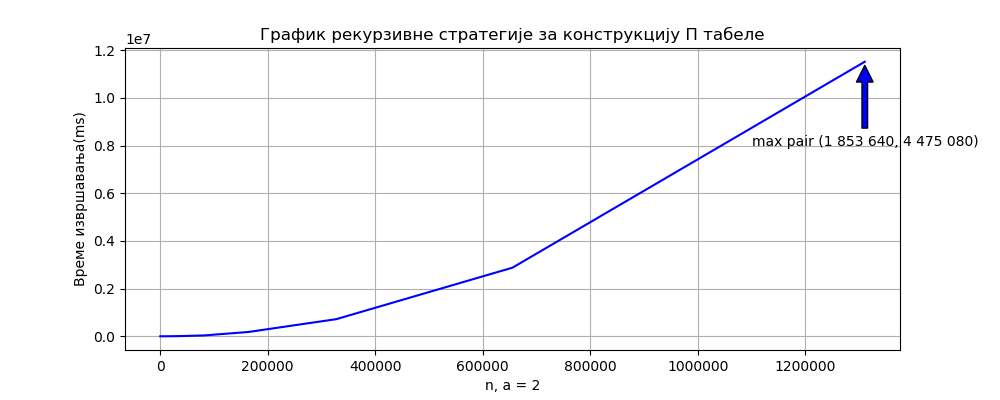
\includegraphics[width=\textwidth]{recursive.png}
	\end{center}
	\caption{График рекурзивне стратегије за конструкцију табеле изгубљених позиција}
	\label{fig:recursive}
\end{figure}

\subsection{Алгебарска стратегија}

За разлику од рекурзиивне стратегије која користи имплицитну рекурзију, алгебарска стратегија рачунајући $ alpha $ и $ beta $ према дефиницијама \eqref{def:alpha}, \eqref{def:beta} користи експлицитну рекурзију (код \ref{lst:algebraic_strategy}). Због тога је укупна временска сложеност конструкције табеле изгубљених позиција $ O(n) $.\\

\lstinputlisting[language=C++, linerange={10-21}, caption=Алгебарска стратегија рачунања табеле изгубљених позиција, label={lst:algebraic_strategy}]{./src/algebraic.cpp}

\leavevmode\\
Графички приказ зависности времена у милисекундама од $ n $ дат је на слици \ref{fig:algebraic}, за $ a = 2 $.

\begin{figure}[H]
	\begin{center}
		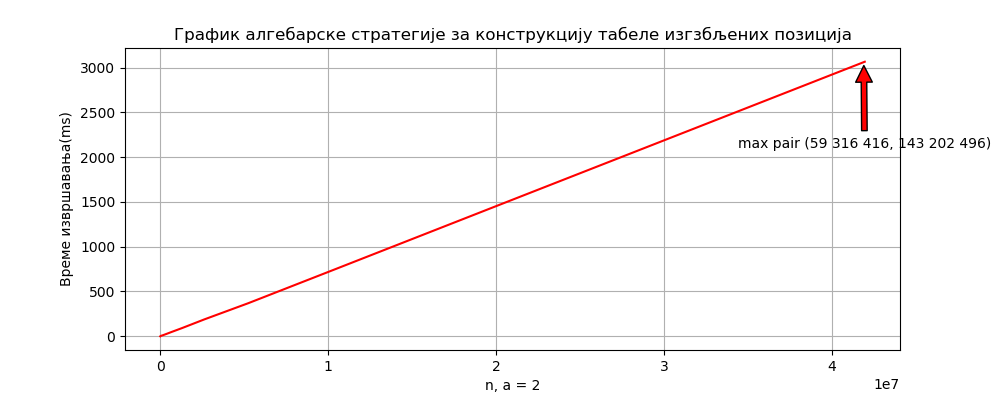
\includegraphics[width=\textwidth]{algebraic.png}
	\end{center}
	\caption{График алгебарске стратегије за конструкцију П табеле}
	\label{fig:algebraic}
\end{figure}

\subsection{Аритметичка стратегија}

За рачунање табеле изгубљених позиција аритметичком стратегијом користи се коначан верижни разломак $ [1, a, a, ...., a] $, што захтева време $ O(n) $ (Функција \verb|alpha_continued_fractions()|) у коду \ref{lst:arithmetic_strategy}).

Потом се формирају низови $ p $ и $ q $ према леми \ref{lemmma:p_q_nizovi}, њихова димензија је највише $ \log(n) $. Стога је врeме за њихово формирање $ O(\log(n)) $ (Функција \verb|p_q_numerations()| у коду \ref{lst:arithmetic_strategy}).

Преостаје још само да $ n $ бројева представимо у $ p $ и $ q $ систему. За њихово представљање у свакој итерацији бинарном претрагом низова $ p $ и $ q $ одређује се са колико цифара треба представити број $ i $, што је у најгорем случају једнако величини низова $ p $ и $ q $, тачније $ \log(n) $. Тако да је сложеност ове бинарне претраге $ O(\log(\log(n))) $. Репрезентација броја $ k $ у $ p $ или $ q $ систему се добија тако што рачунамо количник и остатак при дељењу броја $ k $ са одговарајућом вредности низа $ p $ или $ q $. Уколико имамо остатак, потребно је и њега представити у $ p $ или $ q $ систему. Репрезентација остака у $ p $ или $ q $ систему је позната, тако да је потребно само да је прекопирамо на крај текуће $ p $ или $ q $ репрезентације броја $ k $, не мењајући притом унапред дефинисан број цифара. Сложеност операције копирања једнака је броју елемената који се копира, што је у најгорем случају $ \log(k) - 1 $ цифара. Како имамо $ n $ итерација укупна сложеност представљања првих $ n $ бројева у $ p $ и $ q $ систему захтева $ O(n(\log(\log(n)) + \log(n) - 1)) $ времена (Функцијом \verb|p_system_calculation()| у коду \ref{lst:arithmetic_strategy} представља се $ \_n $ бројева у $ p $ систему, аналогно функцији \verb|q_system_calculation()| у коду \ref{lst:arithmetic_strategy} представља се $ \_n $ бројева у $ q $ систему).

Према томе укупна временска сложеност конструкције табеле изгубљених позиција је $ O(n\log(n)) $

\lstinputlisting[language=C++, linerange={13-84}, caption=Аритметичка стратегија рачунања табеле изгубљених позиција, , label={lst:arithmetic_strategy}]{./src/arithmetic.cpp}

\leavevmode\\
Графички приказ зависности времена у милисекундама од $ n $ дат је на слици \ref{fig:arithmetic}, за $ a = 2 $.

\begin{figure}[H]
	\begin{center}
		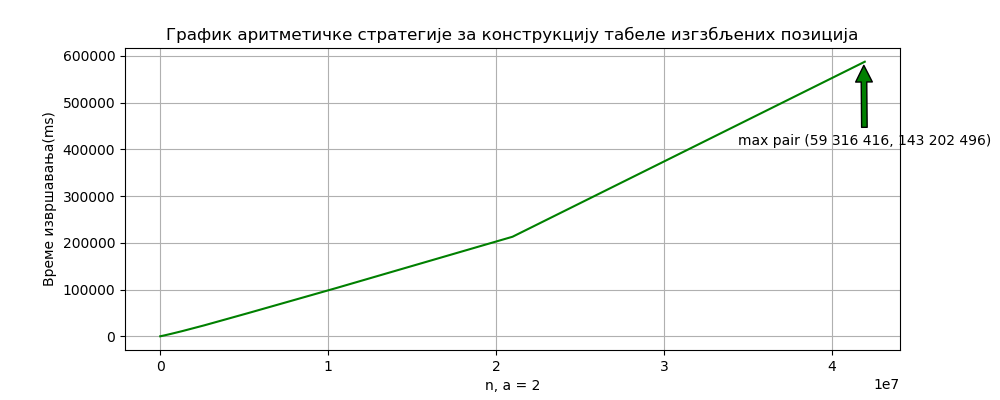
\includegraphics[width=\textwidth]{arithmetic.png}
	\end{center}
	\caption{График аритметичке стратегије за конструкцију табеле изгубљених позиција}
	\label{fig:arithmetic}
\end{figure}

\subsection{Сумиран приказ времена извршавања свих стратегија}

Из претходне анализе, иако је формирање табеле изгубљених позиција алгебарском и рекурзивном стратегијом линеарно, како алгебарска стратегија користи експлицитну рекурзију, може се закључити да је формирање табеле изгубљених позиција овом стратегијом нешто брже, што се може видети и на обједињеним графицима \ref{fig:all} и \ref{fig:algebraicVrecursive}.

\begin{figure}[H]
	\begin{center}
		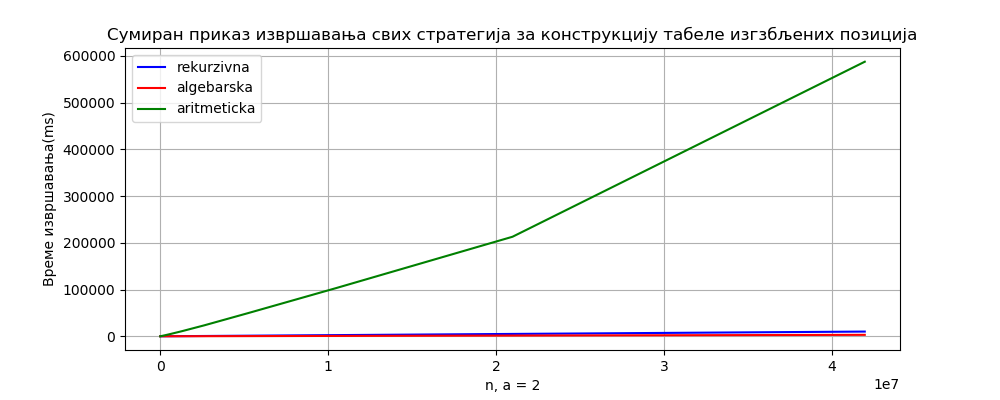
\includegraphics[width=\textwidth]{all.png}
	\end{center}
	\caption{Сумиран приказ извршавања свих стратегија за конструкцију табеле изгубљених позиција}
	\label{fig:all}
\end{figure}

\begin{figure}[H]
	\begin{center}
		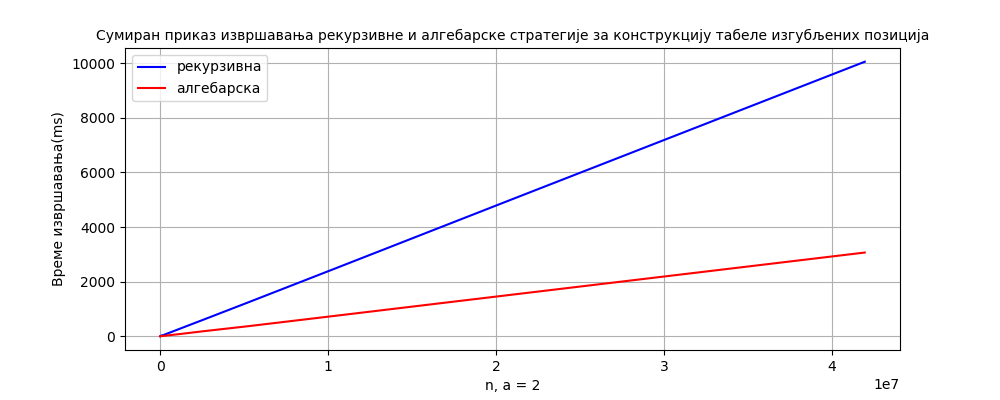
\includegraphics[width=\textwidth]{algebraicVSrecursive.png}
	\end{center}
	\caption{Сумиран приказ извршавања рекурзивне и алгебарске стратегије за конструкцију табеле изгубљених позиција}
	\label{fig:algebraicVrecursive}
\end{figure}

\subsection{Препознавање природе тренутне позиције}

Када имамо израчунате изгубљене позиције, можемо да анализирамо природу тренутне позиције и да одредимо следећу позицију игре.

У коду \ref{lst:recursive_and_algebraic} је за рекурзивну и алгебарску стратегију приказана провера да ли је текућа позиција изгубљена, и ако није функција \textit{reach\_P\_position(vector<int>\& piles)}, која као аргумент прима тренутни број жетона на столу, рачуна следећи пар жетона тако да се достигне изгубљена позиција. За рачунање такве позиције користе се случај 1 и случај 2 из доказа теореме \ref{thm:reukrzivna_strategija}.\\
За аритметичку стратегију, у коду \ref{lst:arithmetic} се најпре ирачунава са колико нула се завршава репрезентација $ R_{p}(x) $. (Функција \verb|number_of_zeros_from_end(_R_{p})|). Уколико се $ R_{p}(x) $ завршава непарним бројем нула, функција \verb|odd_number_of_zeros(vector<int>& piles, vector<int>& R)| рачуна достижну изгубљену позицију, према \ref{item:neparne_nule}. У противном, $ R_{p}(x) $ се завршава парним бројем нула, па се позива функција \verb|even_number_of_zeros(vector<int>& piles, vector<int>& R)| којом се рачуна достижна изгубљена позиција, према \ref{item:parne_nule}.

\lstinputlisting[language=C++, linerange={30-57}, caption= Достизање изгубљене позиције рекурзивном и алгебарском стратегијом, label={lst:recursive_and_algebraic}]{./src/recursive_and_algebraic.cpp}

\lstinputlisting[language=C++, linerange={116-164}, caption= Достизање изгубљене позиције аритметичком стратегијом, label={lst:arithmetic}]{./src/arithmetic.cpp}

\newpage

\section{Закључак}
\label{sec:zakljucak}

Ним је комбинаторна игра за два играча, која је због своје природе привукла разна истраживања на различите теме и стратешке могуности које ова игра пружа. У овој игри нема случајних потеза, као што је бацање коцкица или дељење карата, игра ним припада породици комбинаторних игара које су потпуно одлучиве и чији је главни математички циљ истраживање и рачунање сложености стратегија за победу.
У овој тези кроз примере, поткрепљене математичким доказима приказана су три начина израчунавања изгубљених позиција у Витхофовој игри, варијанти игре ним. Тиме се на три еквивалентна, али доста различита начина описује победничка стратегија у овој игри. Од три имлементиране стратегије, алгебарска се најбрже извршава, иако је и рекурзивна стратегија линеарне временске сложености, она је нешто спорија због рачунања оператора $ \mex $. За разлику од алгебарске и рекурзивне стратегије, код аритметике стратегије приказано је представљање жетона у $ p $ и $ q $ систему, а потом у новом систему и стратегија која је еквивалентна алгебарској и рекурзивној. Занимљиво је да је у случају класичне Витхофове игре победничка стратегија у директној вези са златним пресеком, чиме смо видели и једну примену овог броја у игри. Приказана је статистика извршавања и имплементирана су сва три начина за рачунање табеле изгубљених позиција,  захваљујући којима ће рачунар победити, уколико његов противник не зна како оптимално играти Витхофову игру.  

У овом раду описана је стратегија Витхофове игре у случају нормалног нима. У даљем раду било би занимљиво истражити оптималну стратегију мизерне варијанте Витхофове игре. 

%\csvautolongtable[
%table head=\caption{Времена извршавања у милисекундама конструкције П табеле}\label{tab:calculate_time_n}\\\hline
%\csvlinetotablerow\\\hline
%\endfirsthe
%ad\hline
%\csvlinetotablerow\\\hline
%\endhead\hline
%\endfoot,
%respect all
%]{./src/statistics/csv/calculate_time_n.csv}
%
%\csvautolongtable[
%table head=\caption{Парови жетона П табеле}\label{tab:calculate_piles}\\\hline
%\csvlinetotablerow\\\hline
%\endfirsthead\hline
%\csvlinetotablerow\\\hline
%\endhead\hline
%\endfoot,
%respect all
%]{./src/statistics/csv/calculate_piles.csv}
\newpage
\addcontentsline{toc}{section}{Литература}
\appendix
\bibliography{literatura} 
\bibliographystyle{plain}

\end{document}
